\documentclass[conference,a4paper]{IEEEtran}
\IEEEoverridecommandlockouts
\usepackage[utf8]{inputenc}
\usepackage[T1]{fontenc}
\usepackage[english]{babel}
\usepackage{cite}
\usepackage{amsmath,amssymb}
\usepackage{graphicx}
\usepackage{booktabs}
\usepackage{tikz}
\usetikzlibrary{arrows.meta,positioning}
\usepackage[hidelinks]{hyperref}
\usepackage{xurl}
\graphicspath{{figures/}{../../../figuras/07_cloud_aws/capturas/}}

% Inserts the screenshot if it exists; otherwise draws a labelled placeholder
\newcommand{\captura}[2]{\IfFileExists{capturas/#1}{\includegraphics[width=#2]{capturas/#1}}{\IfFileExists{../../../figuras/07_cloud_aws/capturas/#1}{\includegraphics[width=#2]{../../../figuras/07_cloud_aws/capturas/#1}}{\fbox{\parbox[c][2.2cm][c]{0.95#2}{\centering\small Pending screenshot: \detokenize{#1}}}}}}

\usepackage{float}
\usepackage[section]{placeins}
\begin{document}

\title{Equine Lameness Detection Using Data Mining, Machine Learning and Cloud Computing}

\author{\IEEEauthorblockN{Carlos Josué Barrera Vargas}
\IEEEauthorblockA{Faculty of Data Engineering and Artificial Intelligence\\
Universidad Santo Tomás, Tunja, Colombia\\
Fifth-semester integrative project · Data Mining, Machine Learning and Cloud Computing\\
Repository: \url{https://github.com/Cjoh210/Proyecto_Deteccion_Marcha_Equina}}}

\maketitle

\begin{abstract}
Lameness tends to be the most common health problem in horses, and the problem is that its diagnosis depends entirely on a subjective assessment. This work focuses on the exploratory phase of a system to detect it objectively, and it also intends to work with video in future stages. The CRISP-DM methodology was followed to process information using scientific papers, a catalogue of open datasets and sensor signals from 22 horses with induced lameness. The data mining process showed that the field is moving towards the use of computer vision, while there is a lack of research in Colombia and of datasets that contain video and natural lameness. The signal analysis confirmed that asymmetry in the movement of the head and pelvis reveals lameness, shown with a model validated on new data to test generalization. The complete system was deployed on AWS using Terraform, with a serverless architecture.
\end{abstract}

\begin{IEEEkeywords}
data mining, CRISP-DM, ensemble learning, cloud computing, equine lameness, sustainable development
\end{IEEEkeywords}

\section{Introduction}

Lameness in horses is often the first sign of declining health and a truly costly condition for the sector, because the animal loses time of use while it rests and needs a long and laborious treatment~\cite{nehs2013,usda1998}. Diagnosis is based mainly on observing the animal at trot, and several studies show that veterinarians agree little with each other when lameness is mild~\cite{keegan2010,hammarberg2016}.

Colombia has nearly one million registered horses~\cite{agronegocios2025censo}, and the criollo horse has an important cultural and economic value in regions such as the Eastern Plains and Boyacá. A system that estimates lameness from a phone video would establish a technical assessment standard from which field veterinarians and breeders can benefit. Before building it, this work answers three questions: what has been researched and where the gap lies, what public data are available, and which movement signals reveal a lame horse. With those answers, a predictive model was built and deployed in the cloud as a complete service.

\section{Problem Statement}

Lameness assessment is subjective, and objective methods, such as body-mounted sensors, force plates or motion capture, are expensive or require instrumenting the animal. For this reason they remain out of reach for many breeders and rural veterinarians.

\textbf{Research question.} Is it possible to estimate the probability that a horse is lame from movement data obtainable with accessible technology, in an interpretable way and with a low deployment cost?

\textbf{Users and beneficiaries.} Field veterinarians, who gain an objective second opinion and follow-up over time; breeders and criollo horse associations, who can monitor their animals; and the horses themselves, which receive an earlier diagnosis.

\textbf{Alignment with the SDGs.} The project is linked to SDG 3, Good health and well-being, through the One Health approach, which integrates animal and human health~\cite{un2015}, and to SDG 8, Decent work and economic growth, by reducing losses in a rural sector that generates employment.

\section{Related Work}

Objective lameness assessment has relied on inertial sensors on the head and pelvis, which measure how uneven the vertical displacement is at each step; these measures are related to the clinical examination, although they do not replace it~\cite{keegan2013}. In computer vision, DeepLabCut made it possible to locate anatomical points in video without markers~\cite{mathis2018}, and horse datasets such as Horse-10 and PFERD appeared~\cite{mathis2021,li2024pferd}, together with multi-species pose benchmarks such as AP-10K, APT-36K and Animal Kingdom~\cite{yu2021ap10k,yang2022apt36k,ng2022animalkingdom}. None of them includes clinical lameness labels. Automatic detection is more advanced in cattle, with public databases such as CowScreeningDB~\cite{ismail2024cow}. This work quantifies that gap and proposes a way to close it.

\section{Theoretical Framework}

This work combines data mining, machine learning and cloud computing techniques. This section summarizes those that support the main results.

\subsection{Concepts and acronyms}

\begin{itemize}
\item \textbf{CRISP-DM:} standard data mining methodology with six phases, from problem understanding to deployment~\cite{wirth2000}.
\item \textbf{EDA:} exploratory data analysis with an initial review of statistics and plots.
\item \textbf{IQR:} interquartile range, that is, the distance between the first and third quartiles.
\item \textbf{PCA:} principal component analysis to retain variance.
\item \textbf{SVD:} singular value decomposition, dimensionality reduction of matrices.
\item \textbf{DBSCAN:} density-based clustering algorithm that labels isolated points as noise.
\item \textbf{Apriori and FP-Growth:} algorithms that find items that frequently appear together and generate association rules~\cite{agrawal1994,han2000}.
\item \textbf{KNN:} classifier to assign the class of the nearest cases.
\item \textbf{SVM:} classifier to separate classes with the maximum-margin boundary.
\item \textbf{Cross-validation:} evaluation of a model on several different partitions of the data.
\item \textbf{Grid Search and Random Search:} hyperparameter search.
\item \textbf{ROC-AUC:} measures the model's ability to separate the classes, from 0.5, equal to chance, to 1, perfect.
\item \textbf{API:} interface that allows another program to send data to the system and receive a response.
\item \textbf{SDG:} United Nations Sustainable Development Goals~\cite{un2015}.
\end{itemize}

\subsection{Gait asymmetry}

At trot, the head and pelvis rise and fall twice per stride. In a sound horse both halves are almost equal; when a leg hurts, the animal unloads weight and the movement becomes asymmetric~\cite{keegan2013}. It is measured with the difference between the two lowest points and between the two highest points of the vertical displacement in each stride:

\begin{gather*}
\mathrm{MinDiff} = z_{\min,1} - z_{\min,2} \\
\mathrm{MaxDiff} = z_{\max,1} - z_{\max,2}
\end{gather*}

\subsection{Representation and clustering}

Each abstract is converted into a vector with TF-IDF, which gives weight to the terms that are frequent in a document~\cite{salton1988}:

\[
\mathrm{tfidf}(t,d) = \mathrm{tf}(t,d)\cdot \log\frac{N}{\mathrm{df}(t)}
\]

The matrix is reduced with SVD and clustered with K-Means, which looks for the k centres that minimize the distance of each point to its group~\cite{lloyd1982}. For the dataset catalogue, with mixed numerical and categorical variables, the Gower distance is used, which averages a normalized difference per variable~\cite{gower1971}. Outliers are detected with Isolation Forest, which isolates points with random cuts in the sample~\cite{liu2008}.

\subsection{Ensembles and interpretability}

Random Forest averages many trees trained on different samples and variables, so that it reduces variance~\cite{breiman2001}; Gradient Boosting adds trees over the iterations to correct the error of the previous one~\cite{friedman2001}, and to explain the predictions \textbf{SHAP} is used, which distributes the predictions among the variables according to their average marginal contribution~\cite{lundberg2017}:

\[
\phi_i = \sum_{S \subseteq F \setminus \{i\}} \frac{|S|!\,(|F|-|S|-1)!}{|F|!}\,\big[f(S \cup \{i\}) - f(S)\big]
\]

\subsection{Regularized regression}

Regularization penalizes large coefficients to avoid overfitting. Elastic Net~\cite{zou2005} combines the Lasso penalty, which drives coefficients to zero and selects variables~\cite{tibshirani1996}, with the Ridge penalty; with $\alpha$ = 1 it becomes Lasso and with $\alpha$ = 0, Ridge:

\[
\min_{\beta}\; \lVert y - X\beta \rVert^2 + \lambda \big[ \alpha \lVert\beta\rVert_1 + (1-\alpha) \lVert\beta\rVert_2^2 \big]
\]

\subsection{Serverless computing}

The cloud offers on-demand resources under different service models: IaaS, PaaS and SaaS~\cite{mell2011}. In the serverless model, code runs as functions that are triggered by an event, and they also scale on their own and are billed per execution~\cite{terraform}.

\section{Proposed System}

Fig. 1 shows the complete system. The three sources go into a data lake in the cloud, followed by a mining pipeline that prepares and analyses the data; then a model learns to recognize lameness from gait symmetry measures, and an API delivers the predictions and keeps a history for follow-up.

\begin{figure}[!htb]
\centering
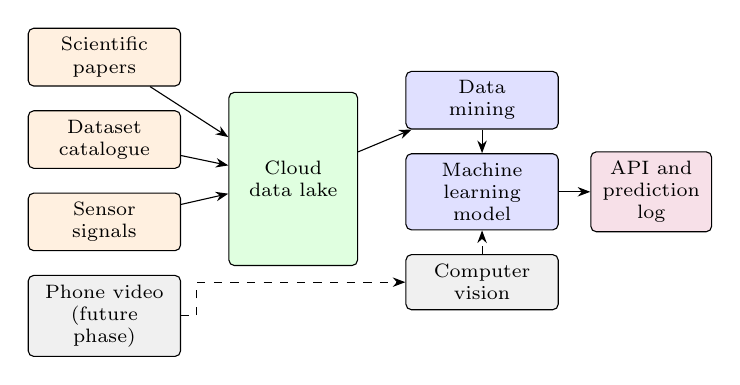
\begin{tikzpicture}[node distance=3mm and 4mm, font=\scriptsize,
  b/.style={draw, rounded corners=2pt, align=center, minimum height=7mm, text width=17mm, fill=#1!12},
  b/.default=blue, >={Stealth[length=1.6mm]}]
\node[b=orange] (api) {Scientific\\papers};
\node[b=orange, below=of api] (cat) {Dataset\\catalogue};
\node[b=orange, below=of cat] (imu) {Sensor\\signals};
\node[b=gray, below=of imu] (vid) {Phone video\\(future phase)};
\node[b=green, right=6mm of cat, yshift=-5mm, text width=14mm, minimum height=22mm] (lake) {Cloud\\data lake};
\node[b, right=6mm of lake, yshift=10mm] (kdd) {Data\\mining};
\node[b, below=of kdd] (ml) {Machine\\learning\\model};
\node[b=gray, below=of ml] (cv) {Computer\\vision};
\node[b=purple, right=4mm of ml, text width=13mm] (srv) {API and\\prediction\\log};
\draw[->] (api) -- (lake); \draw[->] (cat) -- (lake); \draw[->] (imu) -- (lake);
\draw[->, dashed] (vid.east) -- ++(2mm,0) |- (cv.west);
\draw[->] (lake) -- (kdd); \draw[->] (kdd) -- (ml); \draw[->, dashed] (cv) -- (ml); \draw[->] (ml) -- (srv);
\end{tikzpicture}
\caption{General structure of the system.}
\label{fig:sistema}
\end{figure}

\section{Methodology}

The methodology follows the CRISP-DM phases~\cite{wirth2000} and was implemented in six notebooks. This section describes how the data were obtained, prepared and explored.

\subsection{Acquisition}

\textbf{Web scraping of the state of the art.} A Python script queried the OpenAlex API~\cite{priem2022openalex} with five thematic searches: equine lameness, equine gait, sensors, animal vision and pose, and lameness with machine learning in other species, in order to build and keep up to date the resources of the project. With this, 6,472 records were gathered.

\textbf{Dataset catalogue.} Fourteen public datasets were documented with their characteristics and the source link of each one.

\textbf{Sensor signals.} An open dataset was downloaded with 22 Icelandic horses measured sound and with a mild lameness induced in a fore- or hindlimb, recorded with sixteen inertial sensors~\cite{smit2023dataset}.

\subsection{Preparation}

In the corpus, papers repeated across searches were merged, and non-scientific or unrelated documents were also discarded. After cleaning, 4,024 papers remained.

\subsection{Feature engineering}

The raw sensor signals came at scales of millions of samples, which on their own proved not to be useful. The straight-line trot recordings were taken, the vertical displacement of the head, withers, sacrum and hips was computed, and the gait was split into strides in order to standardize the measures. From each stride, measures with real clinical meaning were extracted, so that these variables remained: the difference between the two lowest and the two highest points of each cycle, the range of motion, the regularity of the rhythm and the difference between the hips. The result was a table of 1,817 strides with 27 variables. Missing values were imputed with the median of the same horse and the few physically impossible strides were removed. PCA was applied to this table, where it was clear that several measures are redundant and that sound and lame strides overlap considerably, which anticipates difficulties in the process (Fig. 2).

\begin{figure}[!htb]
\centering
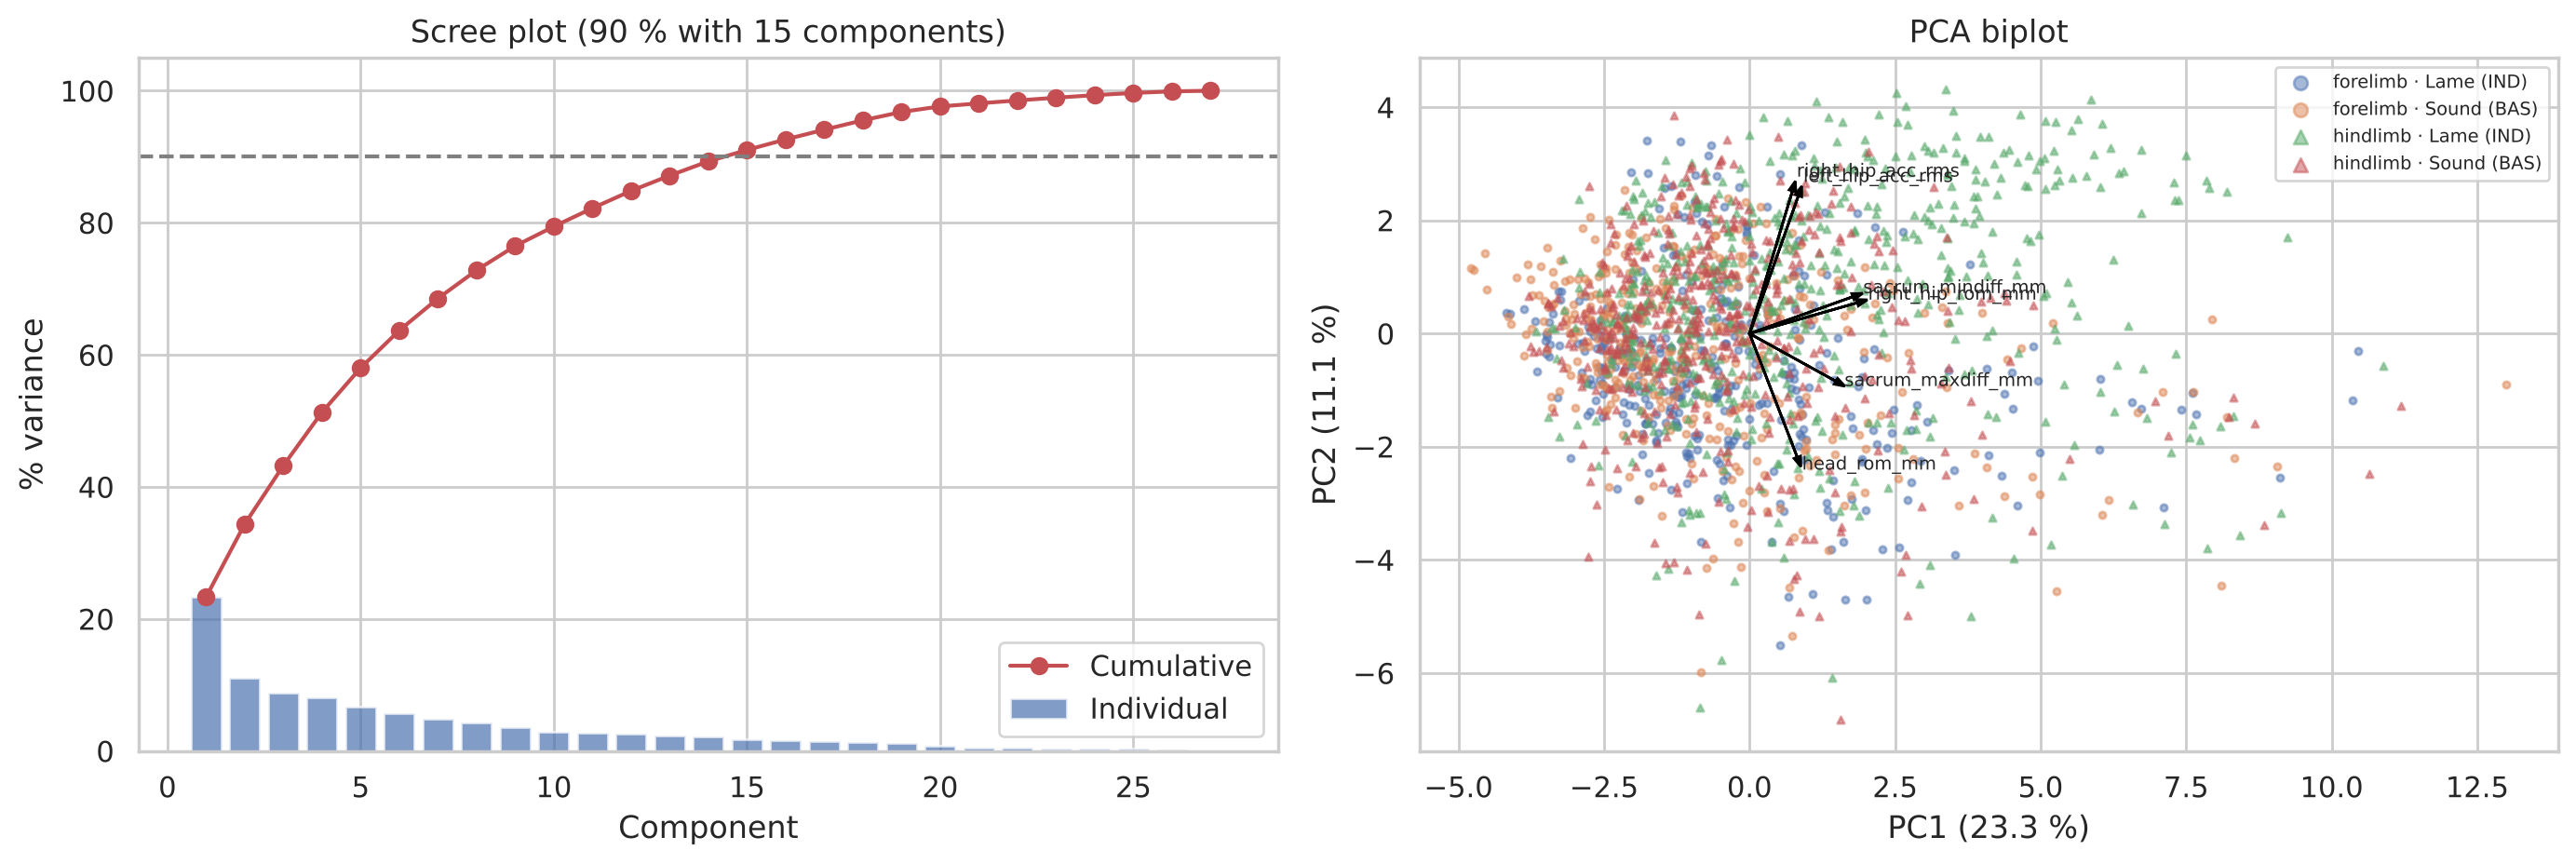
\includegraphics[width=\columnwidth]{imu_pca.png}
\caption{Variance explained by PCA and projection of the strides on the first two components.}
\label{fig:pca}
\end{figure}

\subsection{Exploratory analysis and outliers}

The EDA of the content showed the temporal evolution, countries, journals and impact of the papers. For the sensors, each horse was compared with itself before and after induction using the paired Wilcoxon test, which respects that the strides of the same animal are not independent.

Outliers were interpreted before deciding what to do with them. In the content, the highest-impact papers turned out to be the most widely used computer vision tools in the field, its technological frontier, so they were kept. In the sensors, Isolation Forest was used, and it showed that anomalous strides concentrate in the lame horses, which indicates that the anomaly is the clinical signal itself, so only impossible records and real noise were removed, such as papers unrelated to the study like genetic tests.

\subsection{Unsupervised mining}

The paper abstracts were represented with TF-IDF, then reduced with SVD and clustered with K-Means, choosing the number of groups with four internal metrics and comparing the result with hierarchical clustering and DBSCAN (Fig. 3). The latter was discarded because it left almost half of the papers as noise. In addition, the keywords were analysed with association rules such as Apriori and FP-Growth~\cite{agrawal1994,han2000}, which reached the same frequent itemsets, showing consistency in the process. On the other hand, the dataset catalogue was clustered with the Gower distance and hierarchical clustering, which produced four profiles.

\begin{figure}[!htb]
\centering
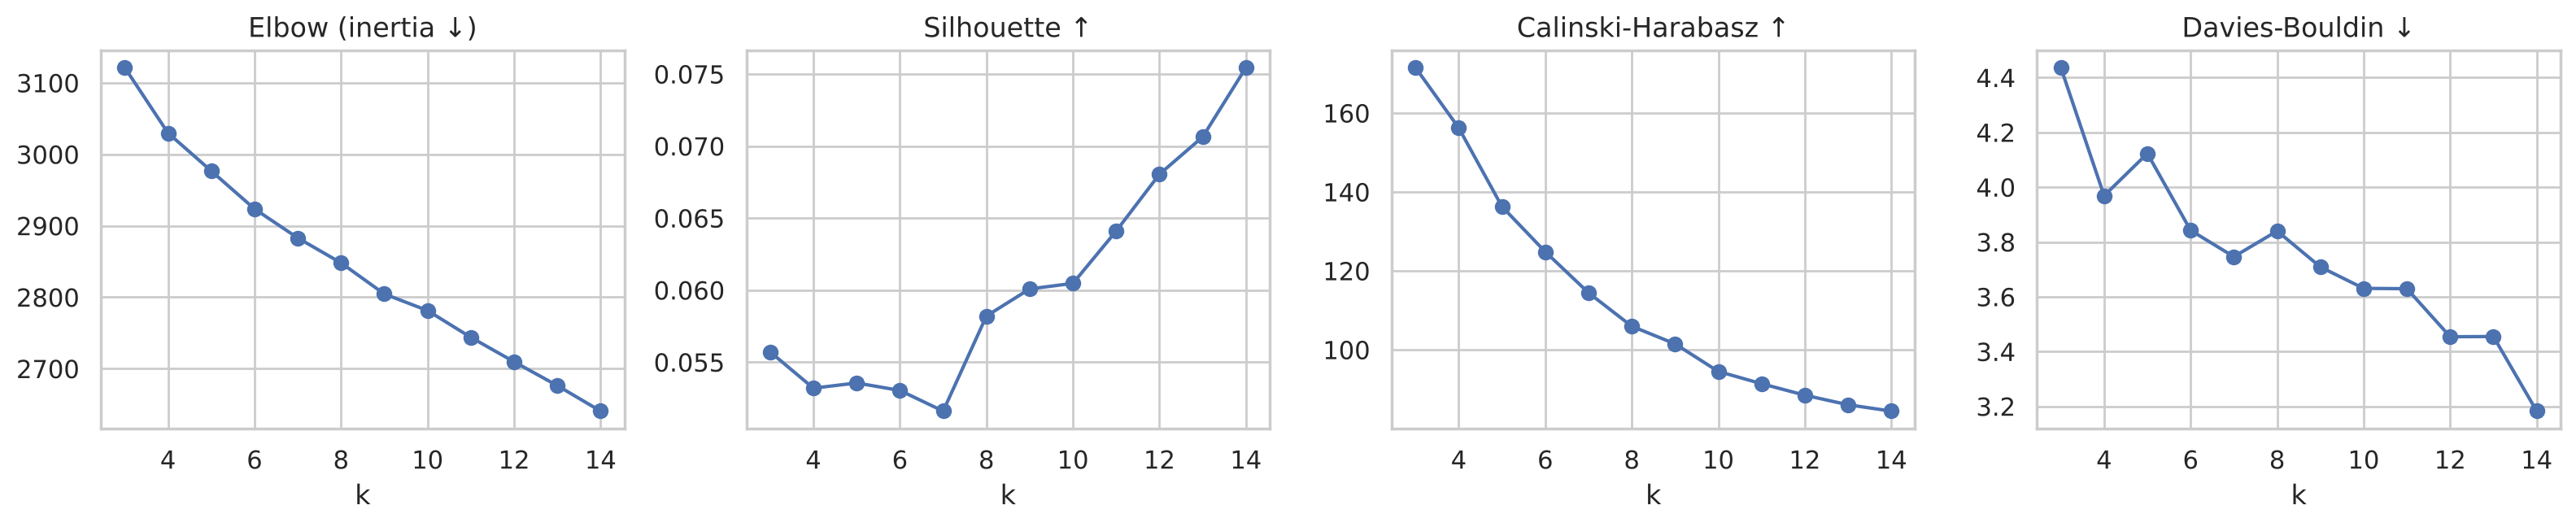
\includegraphics[width=\columnwidth]{art_kmeans_seleccion_k.png}
\caption{Metrics used to choose the number of K-Means clusters.}
\label{fig:k}
\end{figure}

\section{Machine Learning Models}

\subsection{Lameness classifier}

The main model classifies each stride as sound or lame, in such a way that the decision is \emph{validated with horses the model has not evaluated}: strides from the same animal are highly similar, so mixing them between training and test would make the model recognize the horse and not the lameness itself. That is why five complete horses were reserved for the final test, model selection was done with cross-validation grouped by horse, and robustness was checked by leaving one horse out at a time.

All models share an imputation, scaling and classification pipeline, fitted within each partition to avoid information leakage. Logistic regression, KNN and SVM were compared with Random Forest, AdaBoost and Gradient Boosting~\cite{breiman2001}; the hyperparameters were optimized with Grid Search for these models, and Random Search was also used for SVM. The final model could be interpreted with SHAP~\cite{lundberg2017}.

\subsection{Regression of scientific impact}

As a complement, the impact of the papers, measured as citations per year, was modelled from their characteristics: topic, document type, collaboration, open access and thematic profile. Linear, polynomial, Ridge, Lasso and Elastic Net regression were compared~\cite{tibshirani1996,zou2005}, with Grid Search over the regularization strength, and a Random Forest as reference, with the goal of understanding which type of work comes to have more influence in the field.

\section{Cloud Architecture}

\subsection{Selection and justification}

AWS was chosen for a public cloud deployment. The service model used is mainly \emph{FaaS} and \emph{PaaS}, using Lambda functions and managed services, because of the intermittent nature of the load, which repeats its cycle weekly when it is active. For the same reason, on-demand DynamoDB was chosen.

\subsection{Components}

The architecture in Fig. 4 has four blocks. In \emph{ingestion}, EventBridge triggers a Lambda every week that runs the web scraping, with the API key stored encrypted. The \emph{data lake} in S3 is organized into \textbf{raw}, \textbf{processed} and \textbf{models} zones, with encryption and versioning, and its lifecycle archives old data. \emph{Analytics} uses Glue and Athena to query the data with SQL directly on S3. To interact with the system, an HTTP API triggers a Lambda packaged as a Docker image with scikit-learn; it loads the model from S3 and stores each prediction in DynamoDB, which makes it possible to follow the evolution of each horse. CloudWatch is also enabled to send email alerts, together with a monthly budget to avoid cost overruns.

\begin{figure}[!htb]
\centering
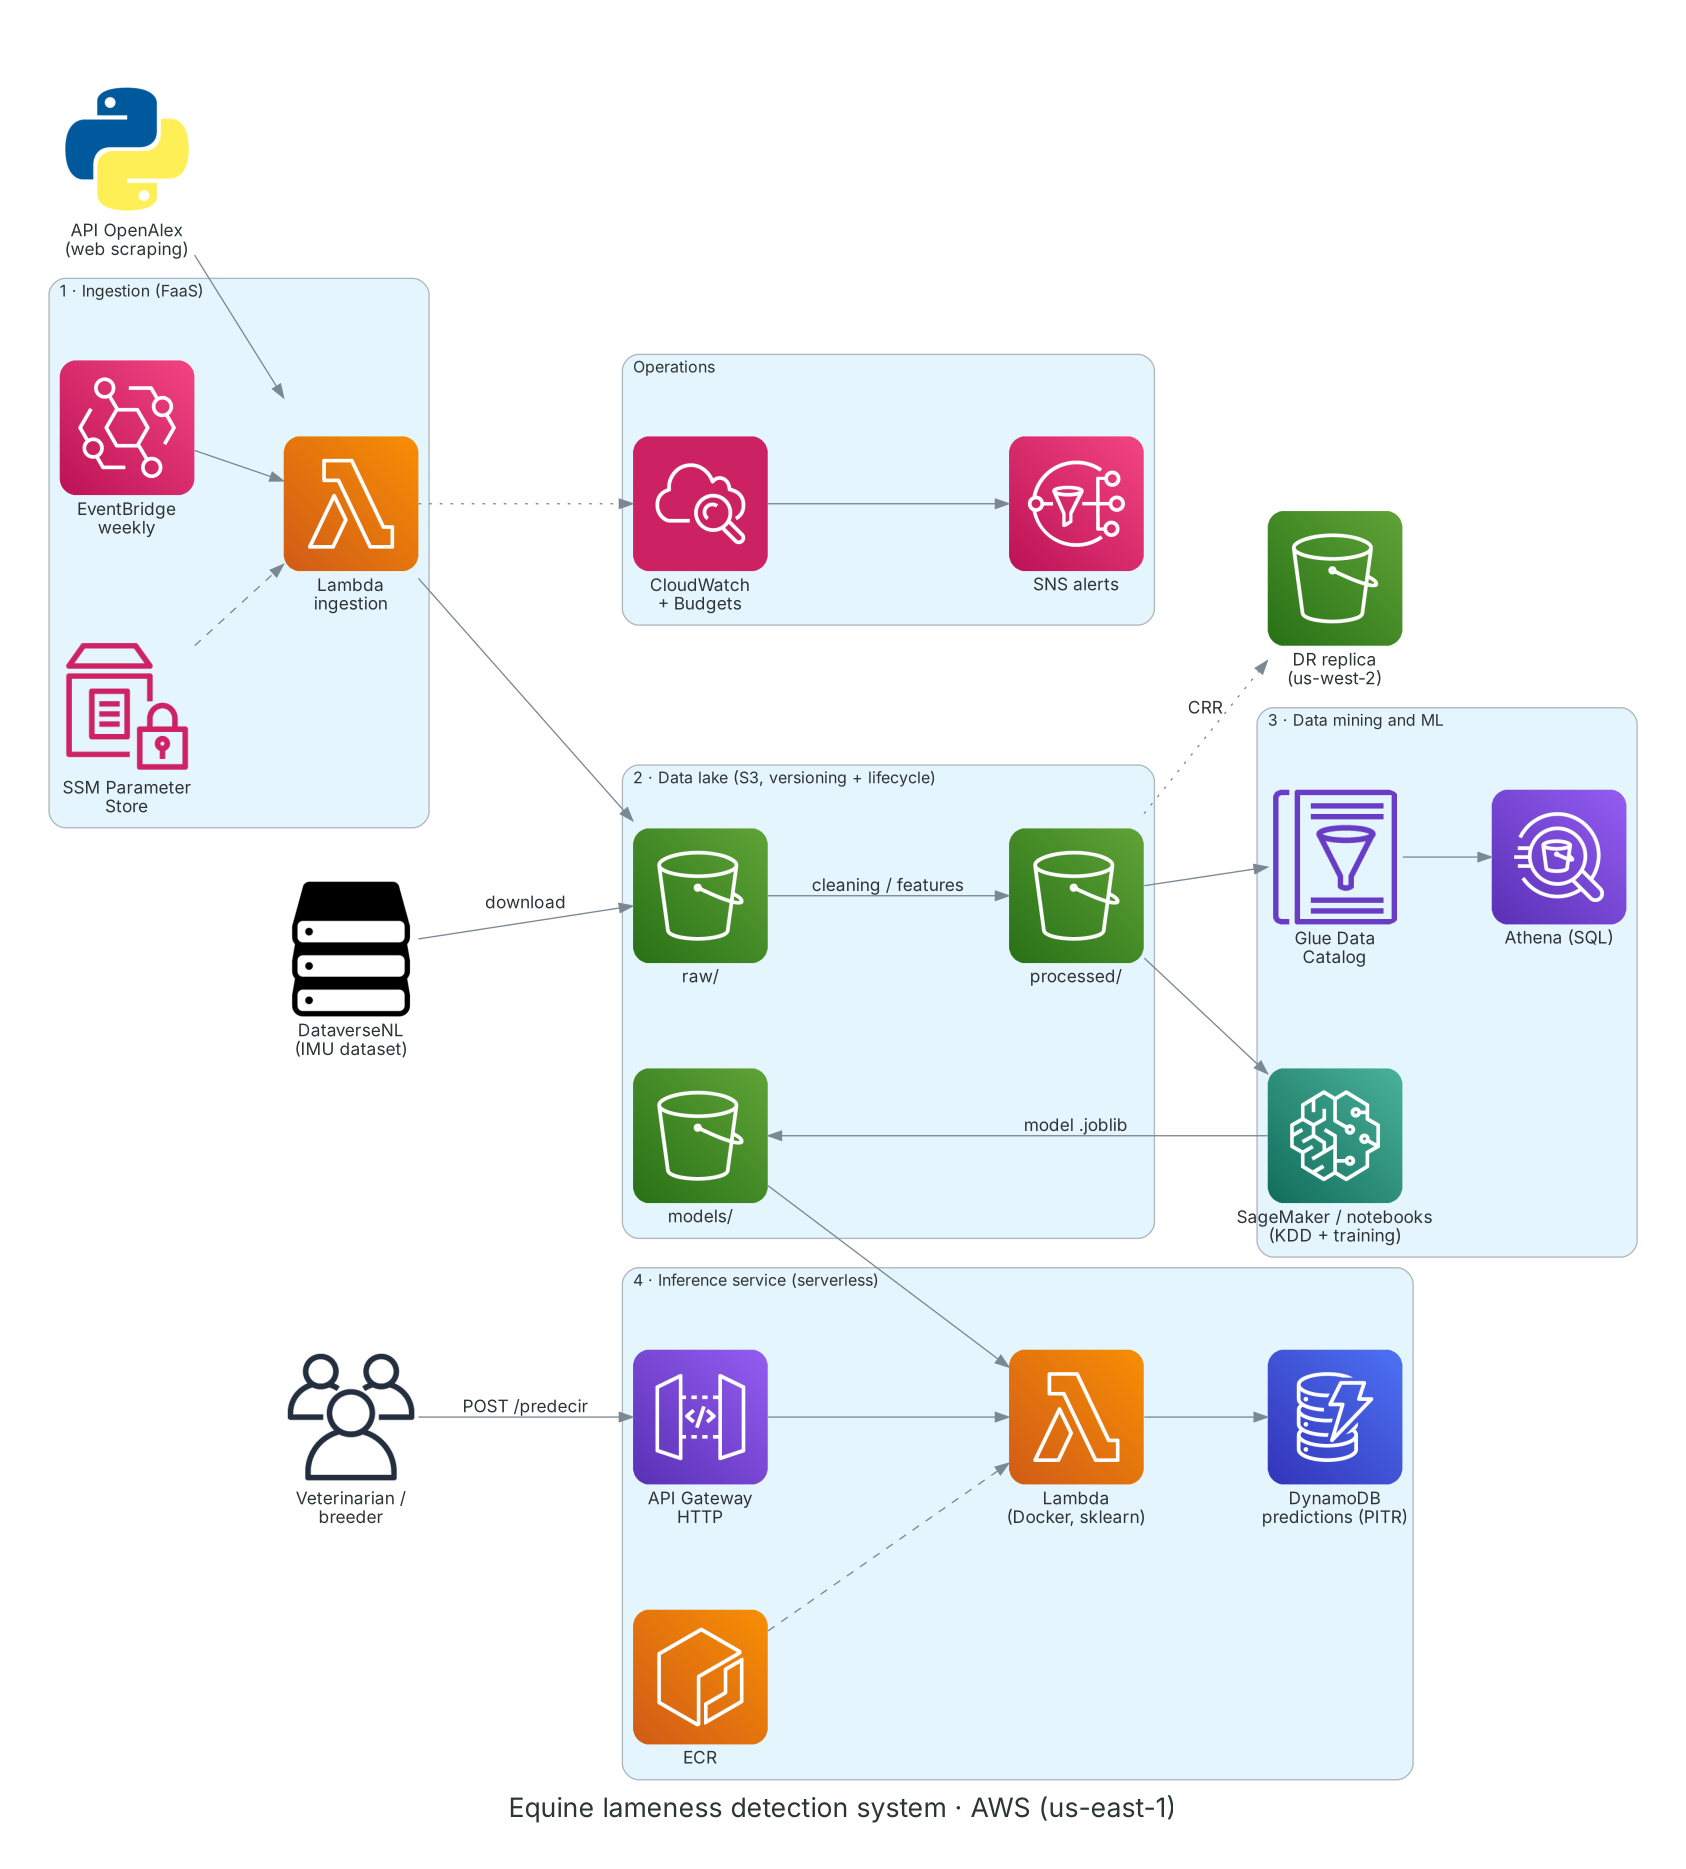
\includegraphics[width=\columnwidth]{arquitectura_aws.png}
\caption{System architecture on AWS.}
\label{fig:aws}
\end{figure}

\subsection{Scalability and recovery}

The services used scale on their own with demand and run in several availability zones, so it was not necessary to configure autoscaling or load balancing. To recover data, S3 keeps versions of each file and DynamoDB can be restored to any point in the last 35 days; in addition, since everything is in Terraform, the infrastructure can easily be recreated.

\subsection{Infrastructure as code and deployment}

The infrastructure was written in Terraform~\cite{terraform} and deployed on a personal AWS account (Fig. 5). The ingestion function runs in the cloud and stores the same corpus obtained locally (Fig. 6). On its first run the function ran out of memory, which was fixed by writing the results to disk incrementally. The incident shows the value of testing the deployed system and not only the code.

\begin{figure}[!htb]
\centering
\captura{terraform_apply.png}{\columnwidth}
\caption{Infrastructure deployment with Terraform.}
\label{fig:apply}
\end{figure}

\begin{figure}[!htb]
\centering
\captura{s3_openalex.png}{\columnwidth}\\[2mm]
\captura{athena_consulta.png}{\columnwidth}
\caption{Corpus stored in S3 by the weekly ingestion and SQL query in Athena on the sensor data.}
\label{fig:ingesta}
\end{figure}

\subsection{End-to-end integration}

Fig. 7 shows the complete operation of the system: a request with the measures of five strides of a horse reaches the API, the Lambda applies the model and responds with the probability of lameness, and the prediction is stored in DynamoDB.

\begin{figure}[!htb]
\centering
\captura{api_respuesta.png}{\columnwidth}\\[2mm]
\captura{dynamodb_items.png}{\columnwidth}
\caption{Inference API response and prediction stored in DynamoDB.}
\label{fig:api}
\end{figure}

\section{Results}

\subsection{State of the art}

Scientific output grows constantly and, in recent years, computer vision has become the dominant research approach over traditional clinical studies (Fig. 8). Clustering identified eight research lines that separate an older clinical group from a more technological one, recent and with higher impact, formed by pose estimation, vision, sensors and detection in cattle (Fig. 9). The association rules showed that animal pose methods are inherited from human pose methods and that automatic lameness detection has been developed mostly in dairy cows. The gap revealed by the research is that, of the works that combine horse, lameness and computer vision, only one has authors in Colombia.

\begin{figure}[!htb]
\centering
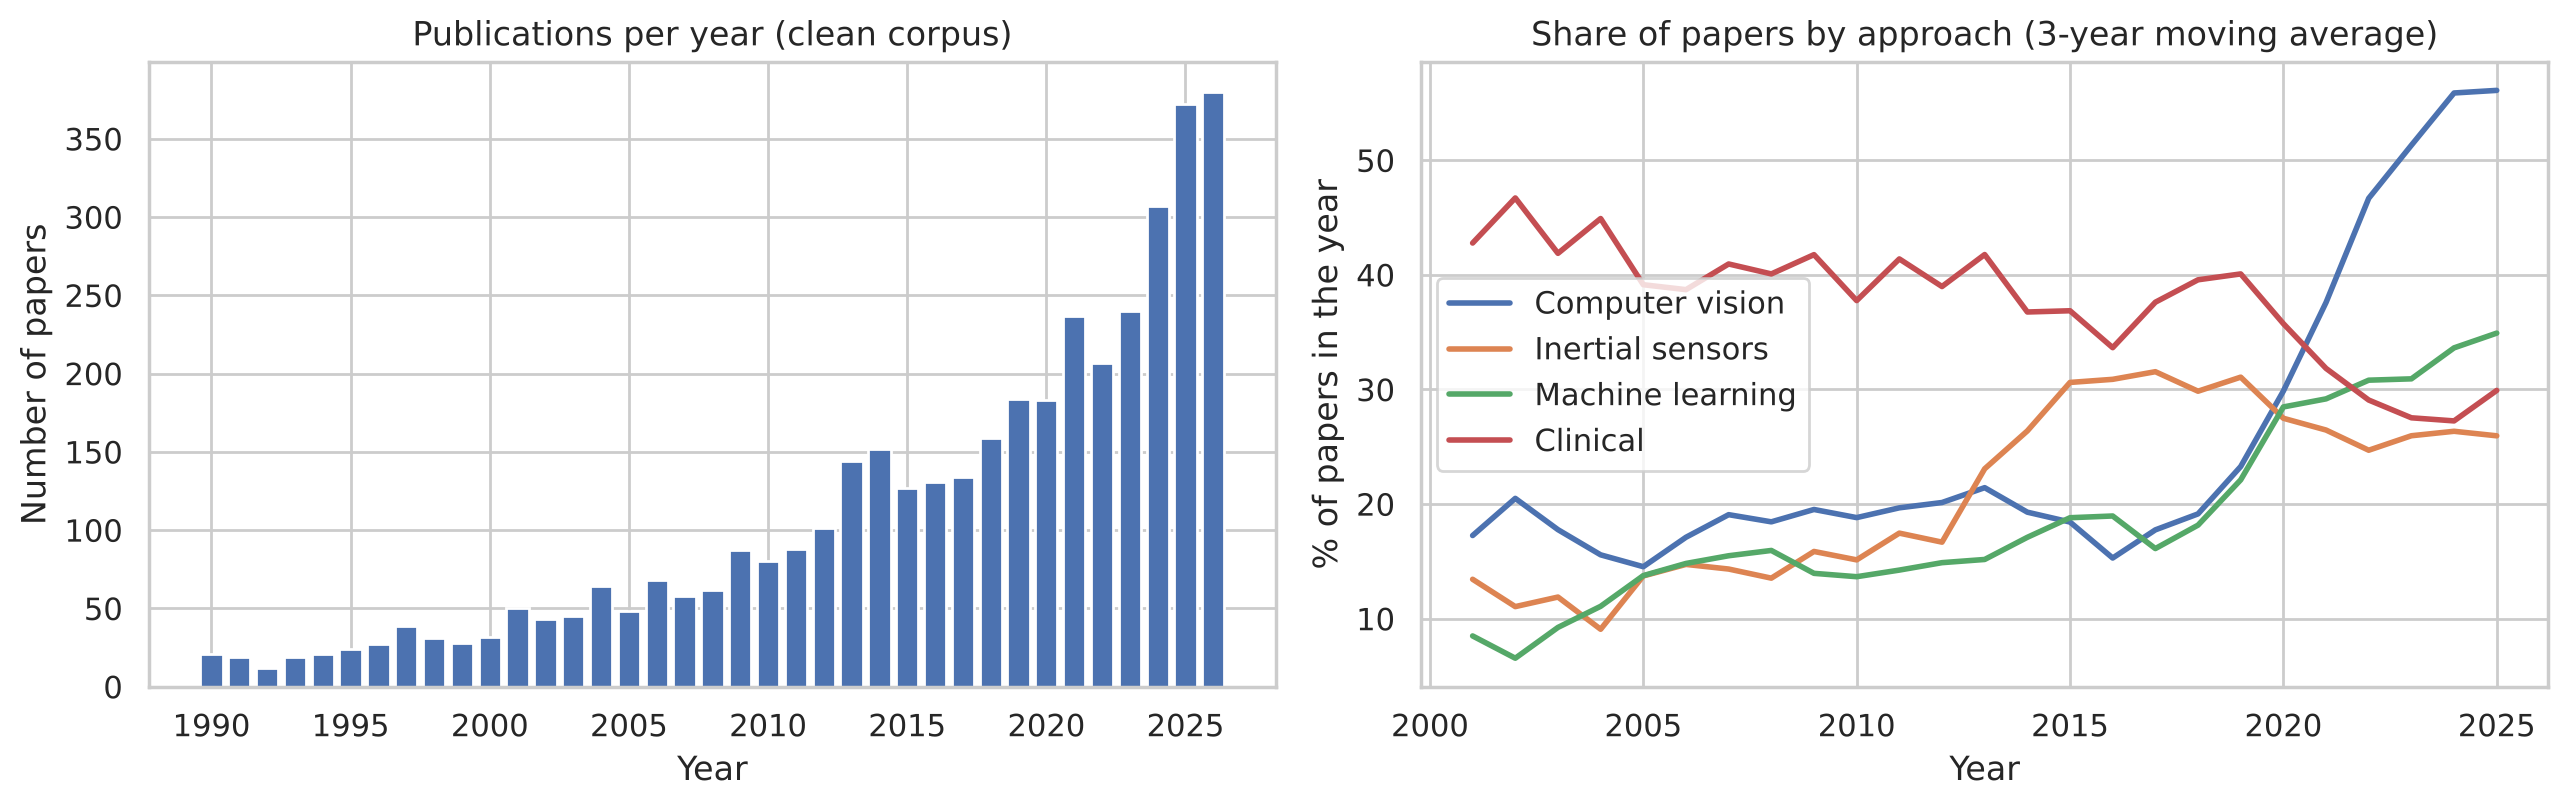
\includegraphics[width=\columnwidth]{art_tendencia_anual.png}
\caption{Publications per year and share of papers by approach. The year 2026 is incomplete.}
\label{fig:tendencia}
\end{figure}

\begin{figure}[!htb]
\centering
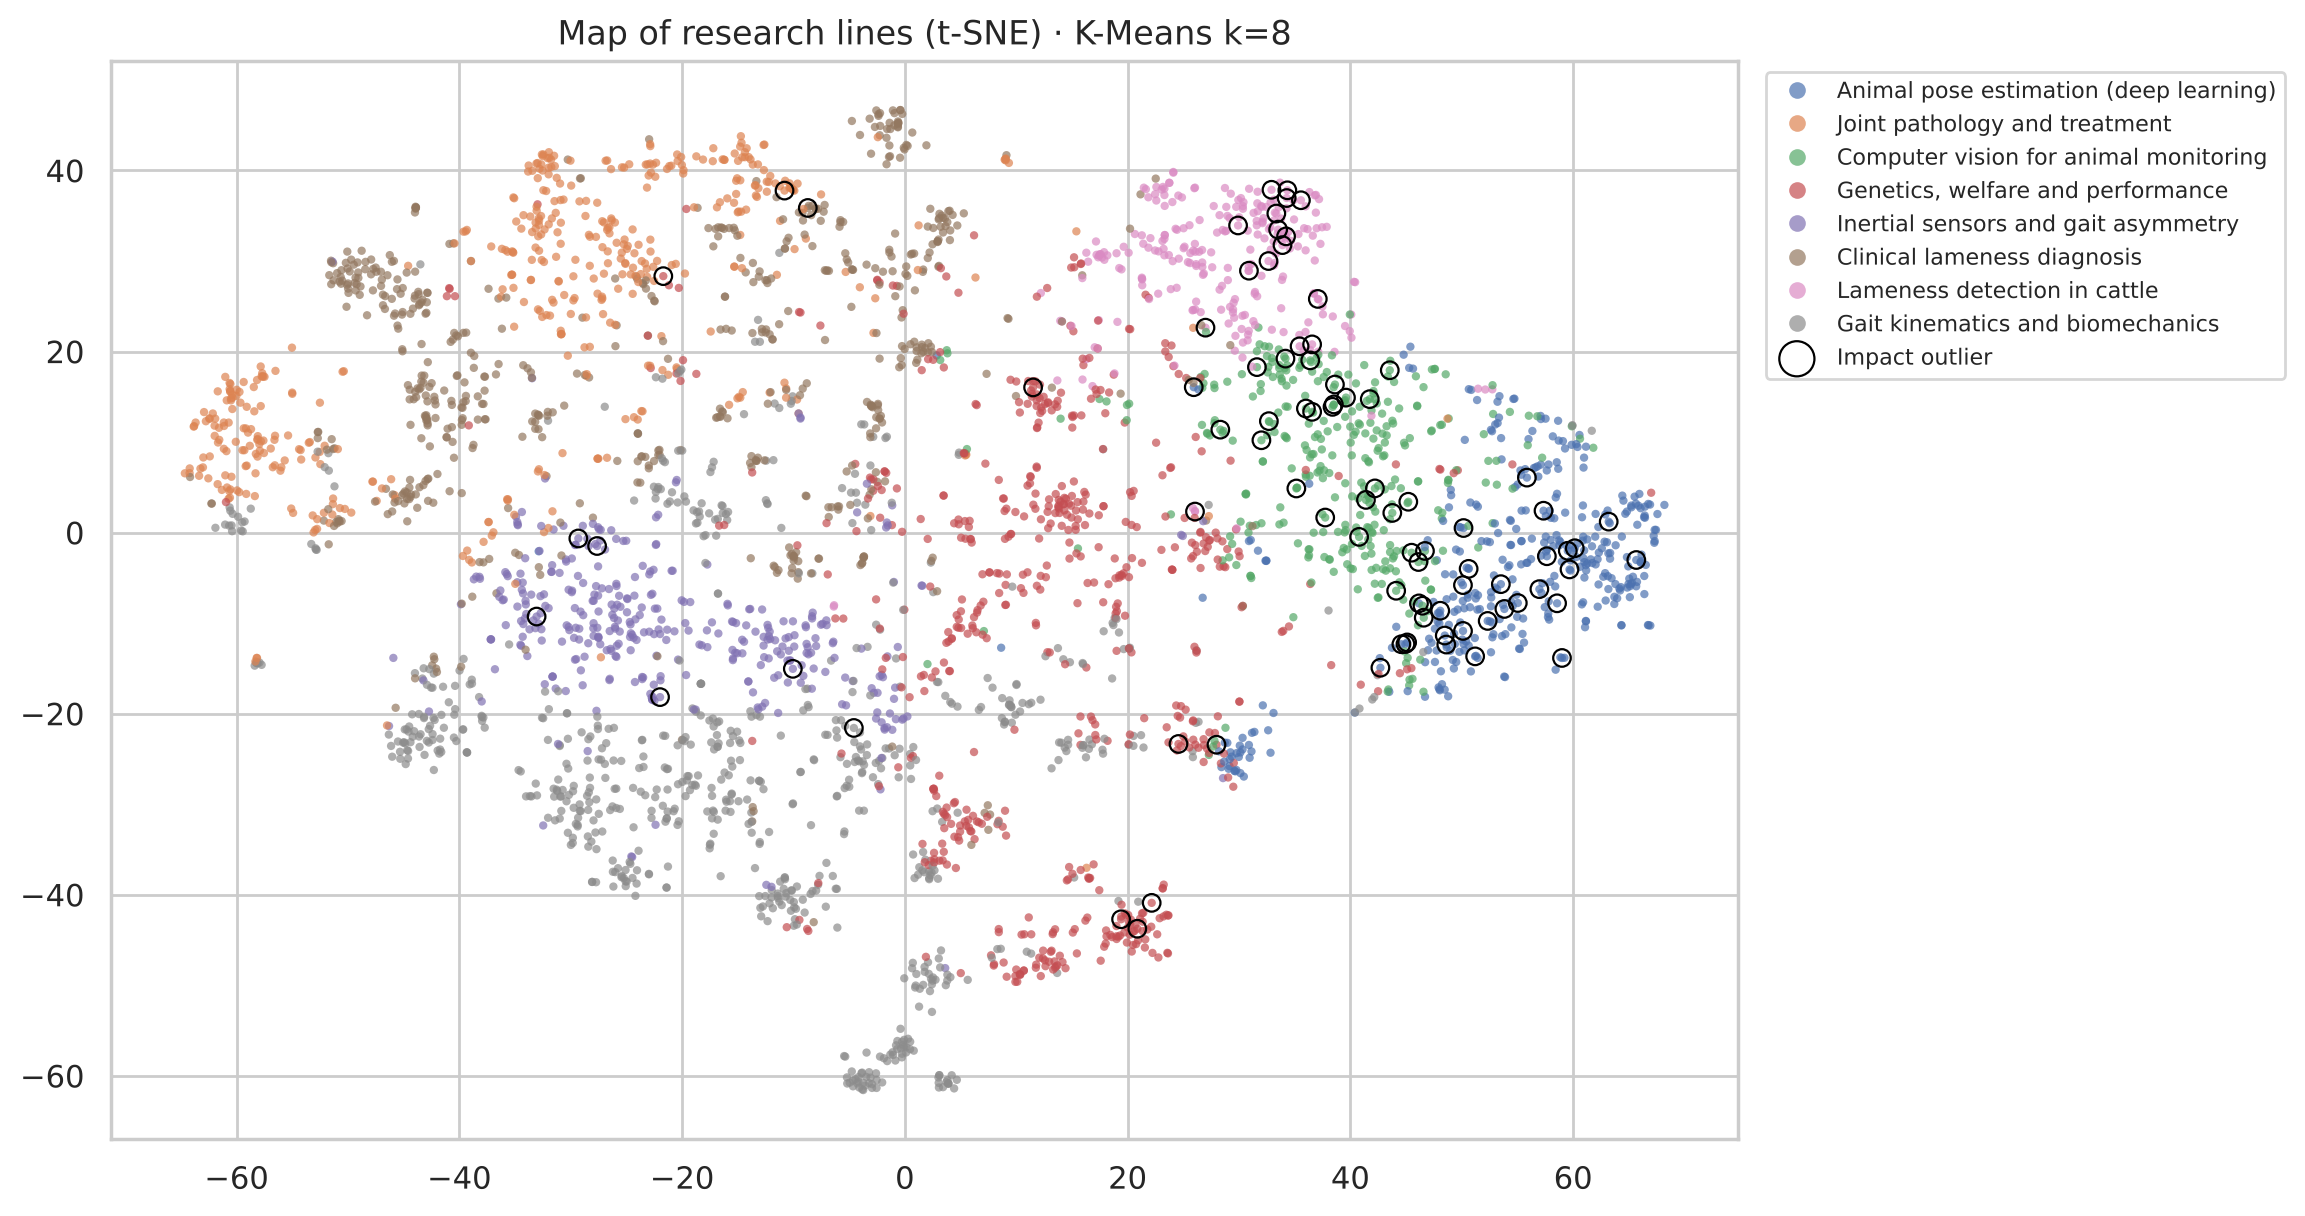
\includegraphics[width=\columnwidth]{art_tsne_clusters.png}
\caption{Map of the research lines found by clustering. Black circles mark papers with outlying impact.}
\label{fig:tsne}
\end{figure}

\subsection{Available datasets}

The catalogue was organized into four profiles: horse motion capture, sensors with lameness labels, pose images and videos with anatomical keypoints. No public dataset combines horse video with lameness labels (Fig. 10). This defines the strategy for a later vision phase: learn to locate the anatomical keypoints with Horse-10 or AP-10K, check the trajectories against the PFERD motion capture and apply the classifier of this work.

\begin{figure}[!htb]
\centering
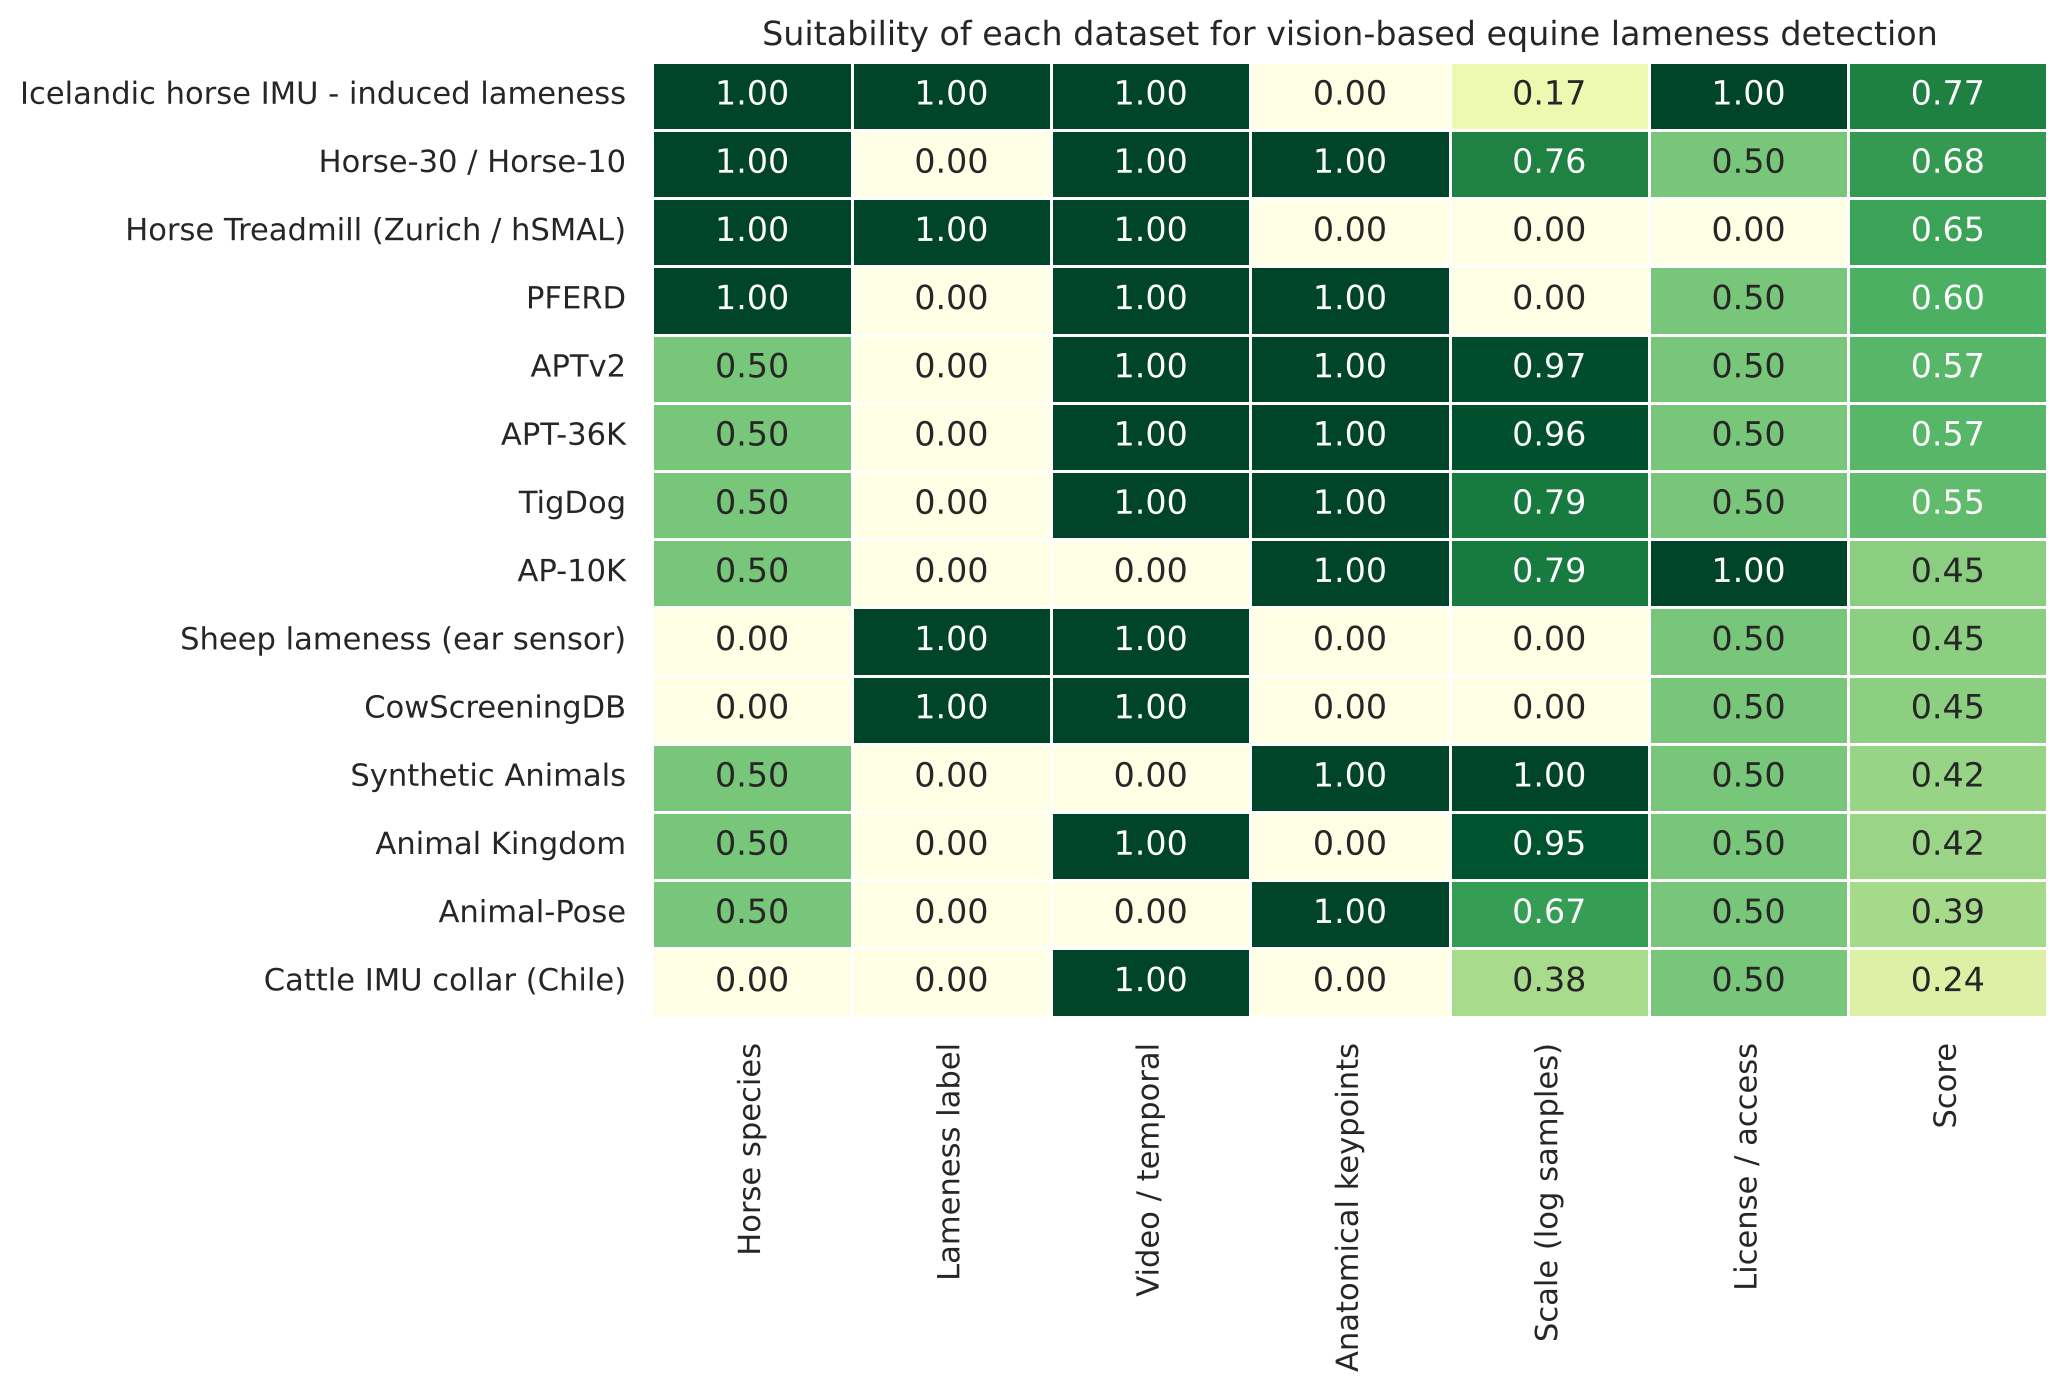
\includegraphics[width=0.9\columnwidth]{cat_matriz_aptitud.png}
\caption{Suitability of each public dataset for the goal of the project.}
\label{fig:aptitud}
\end{figure}

\subsection{Gait signals}

When each horse was compared with itself, forelimb lameness almost doubled head asymmetry, while hindlimb lameness increased sacrum asymmetry and the difference between the hips, with statistically significant differences (Figs. 11 and 12). Clinical practice describes this pattern as the horse raising its head when it bears weight on a painful front leg, and its hip when the pain is behind. The response varies between individuals, and some horses are asymmetric even when sound. Clustering the horses confirmed it: it largely separated the sound from the lame, except precisely for those individuals. That is why a fixed threshold does not do the job.

\begin{figure}[H]
\centering
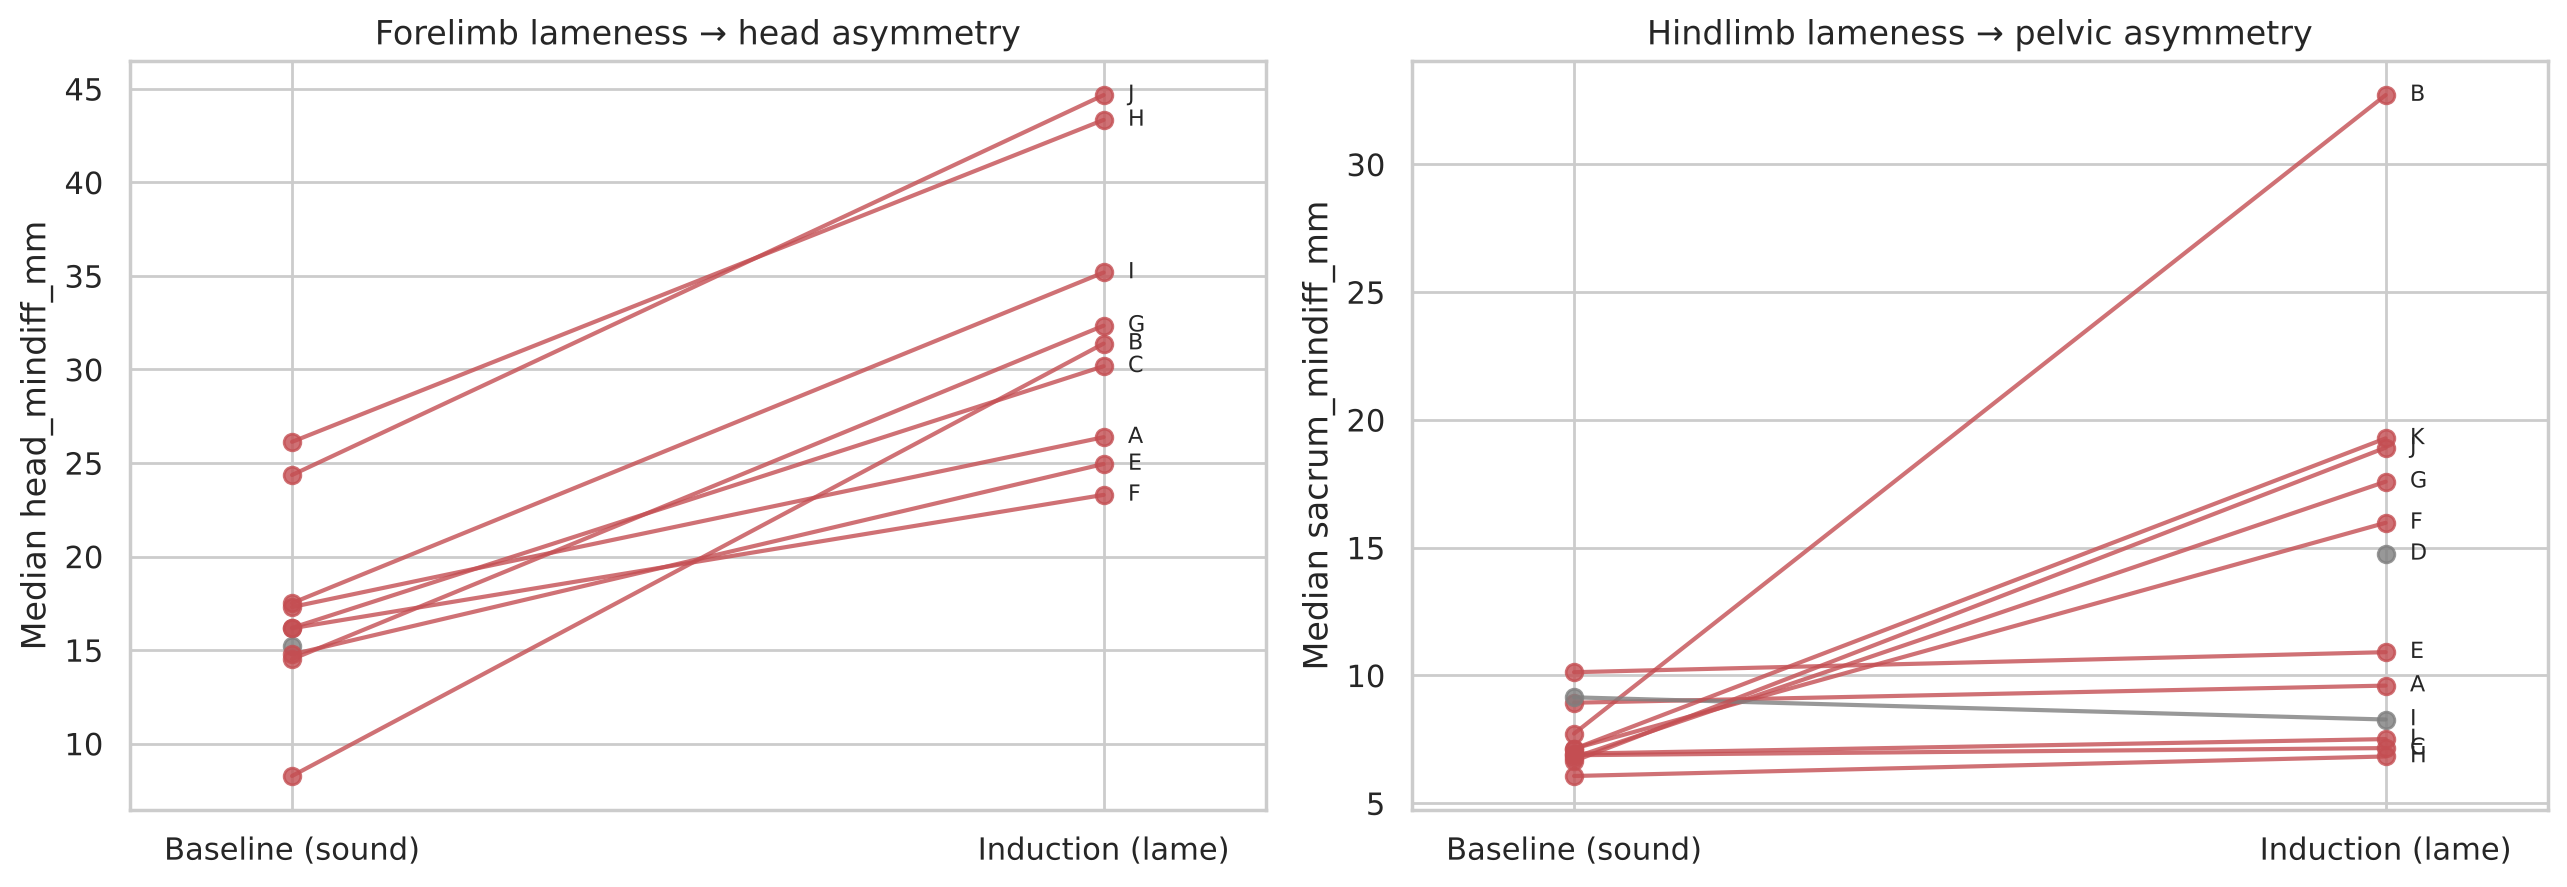
\includegraphics[width=\columnwidth]{imu_pareado_caballos.png}
\caption{Change in each horse's asymmetry between the sound condition and induced lameness.}
\label{fig:pareado}
\end{figure}

\begin{figure}[H]
\centering
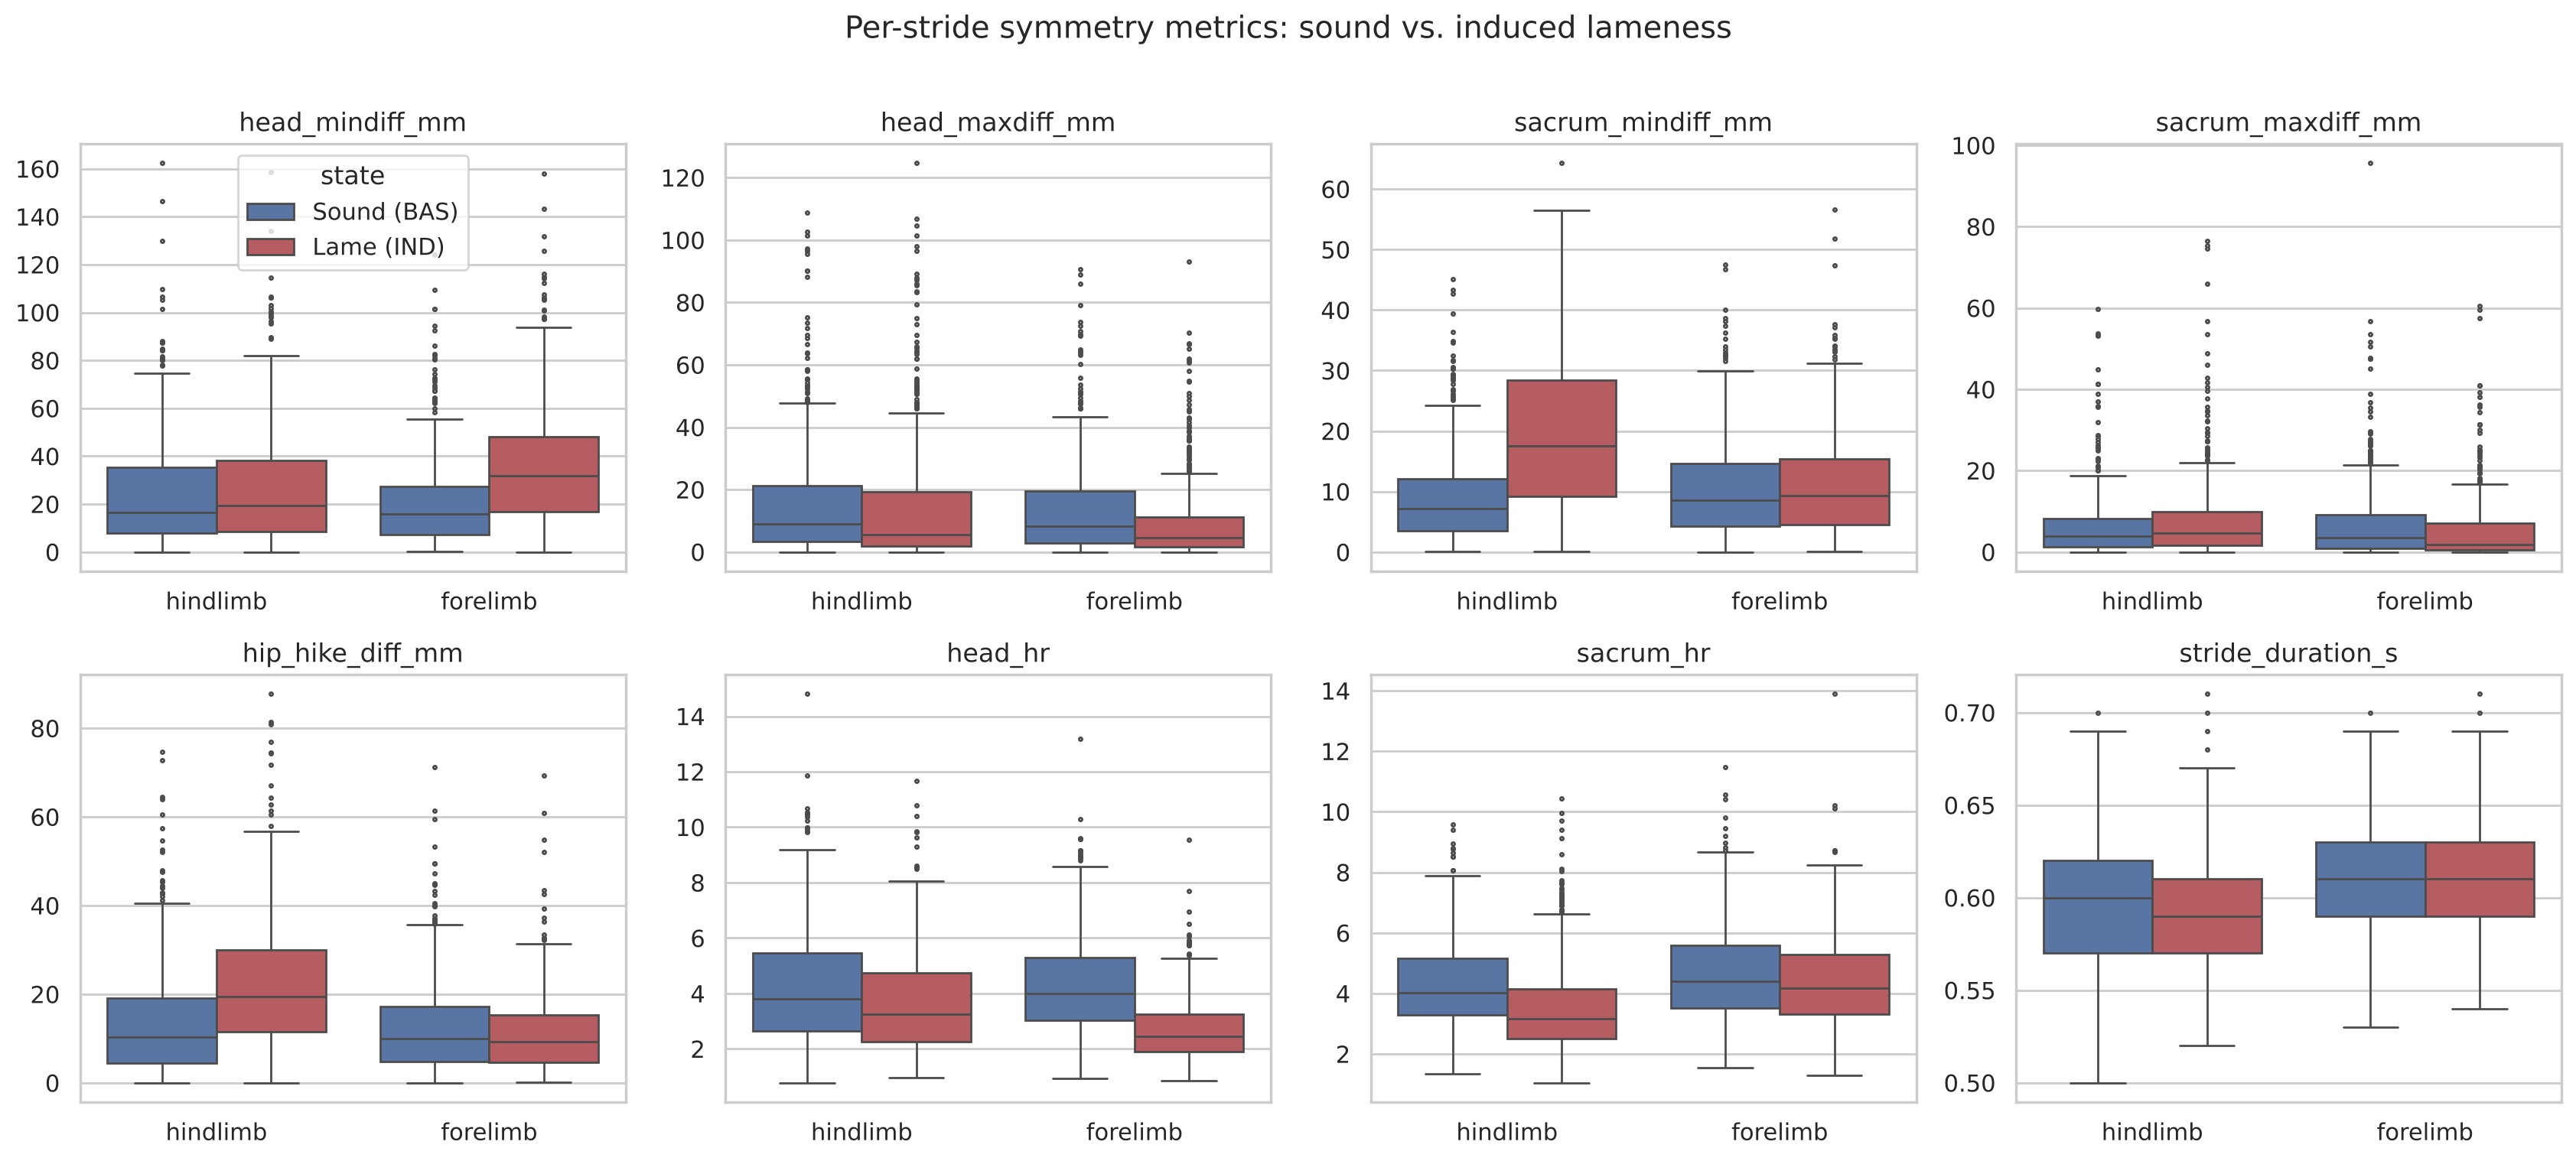
\includegraphics[width=\columnwidth]{imu_boxplots.png}
\caption{Distribution of per-stride symmetry metrics in sound horses and horses with induced lameness, by type of lameness.}
\label{fig:box}
\end{figure}

\subsection{Lameness classifier}

Table I summarizes the results. In cross-validation the models were close to each other, and Random Forest was the best after optimization, so it was chosen as the final model for its performance, its exact interpretability with SHAP, besides having a low computational cost. On the five test horses it reached a ROC-AUC of 0.71, the same value obtained when leaving one horse out at a time, and when averaging the strides of each trot trial it was correct in seven out of nine (Fig. 13). Gradient Boosting performed slightly better on the test set, but it was not chosen, because the model is selected with validation and not by looking at the test set. SHAP shows that the model relies on sacrum asymmetry, the regularity of head movement and the difference between the hips, the same markers a veterinarian uses (Fig. 14). The performance is moderate, as expected with mild lameness evaluated on new horses, and it is an honest estimate of how the system would work in practice.

\begin{table}[H]
\centering
\caption{Classification with horse-grouped validation (ROC-AUC)}
\label{tab:ml}
\begin{tabular}{lcc}
\toprule
Model & Cross-validation & Test \\
\midrule
Logistic regression & 0.67 & 0.68 \\
Optimized SVM & 0.68 & 0.69 \\
Optimized Gradient Boosting & 0.63 & 0.72 \\
\textbf{Optimized Random Forest} & \textbf{0.67} & \textbf{0.71} \\
\bottomrule
\end{tabular}
\end{table}

\begin{figure}[!htb]
\centering
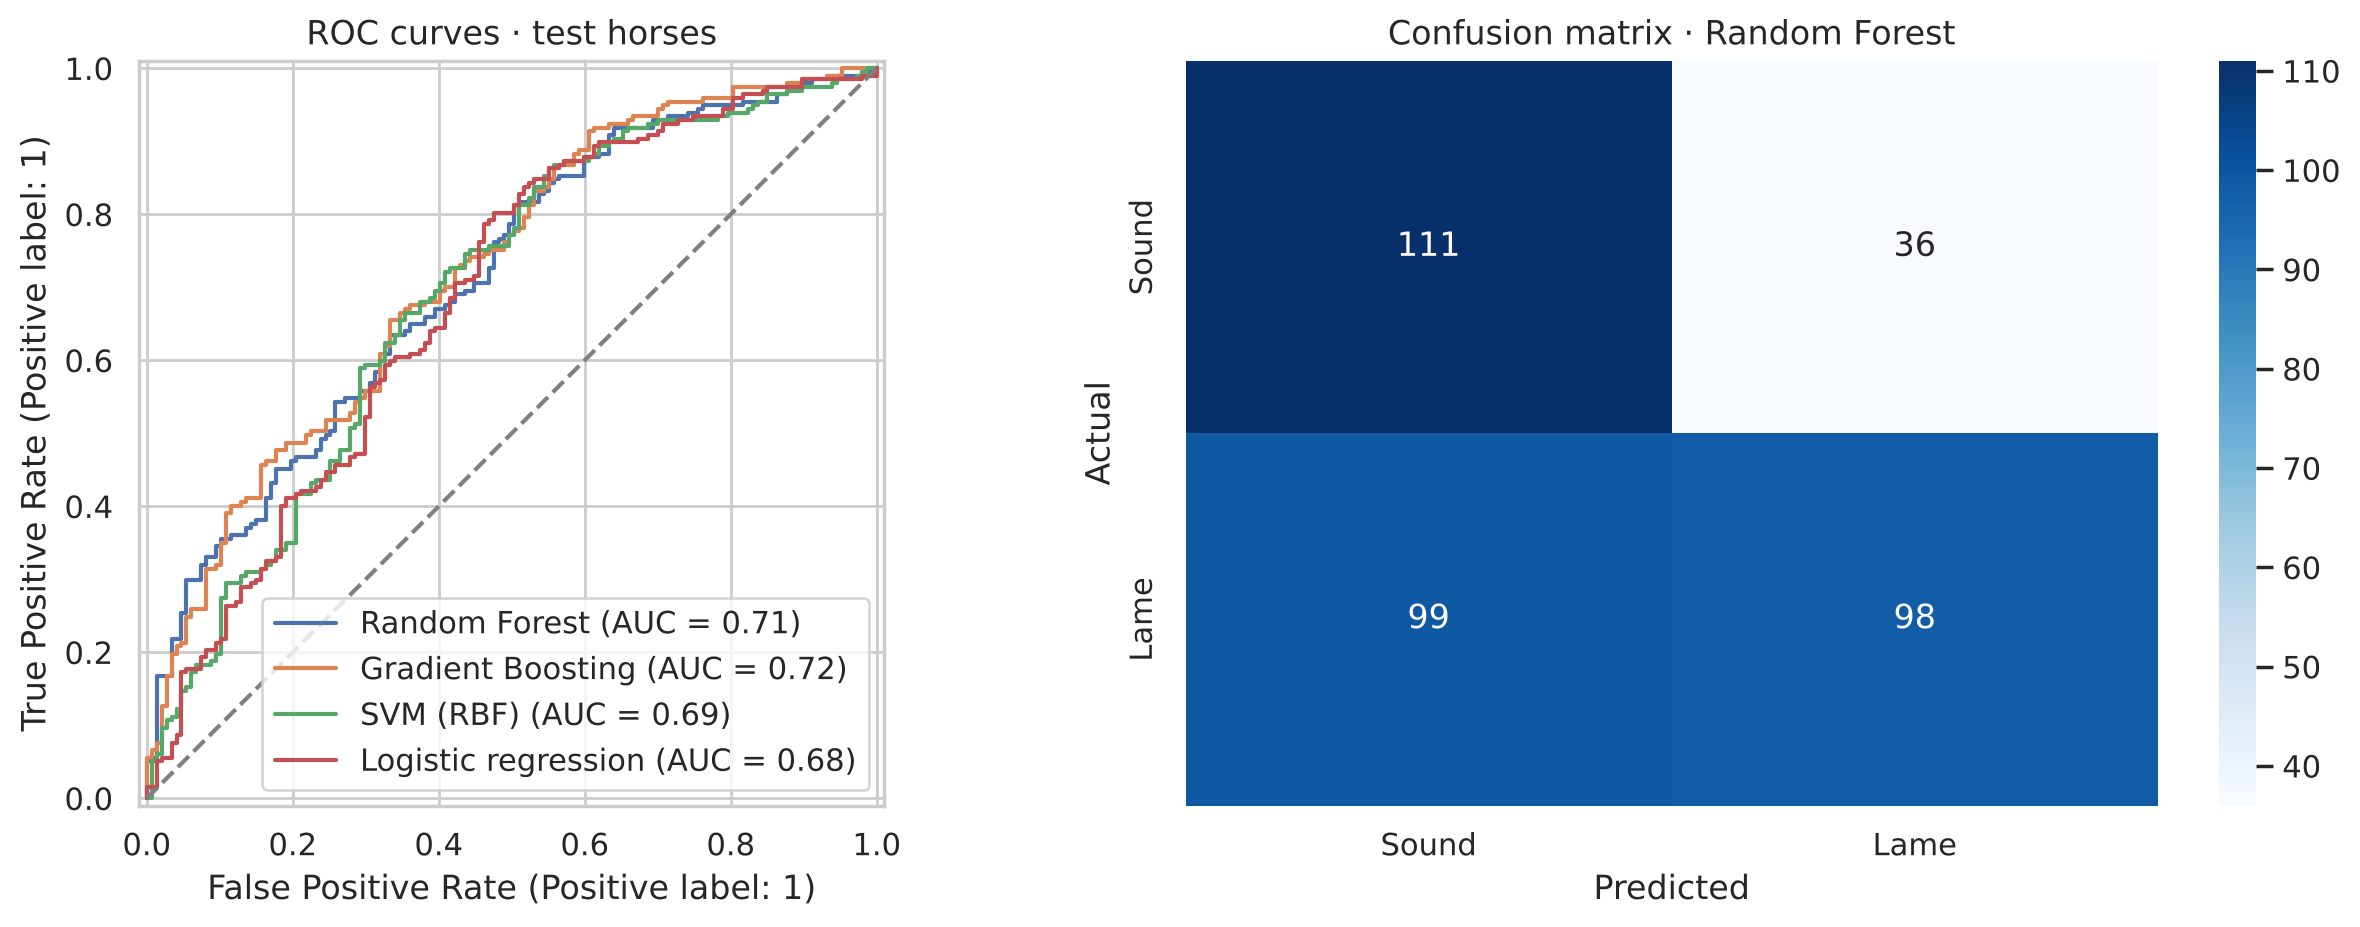
\includegraphics[width=\columnwidth]{ml_roc_confusion.png}
\caption{ROC curves on the test horses and confusion matrix of the final model.}
\label{fig:roc}
\end{figure}

\begin{figure}[!htb]
\centering
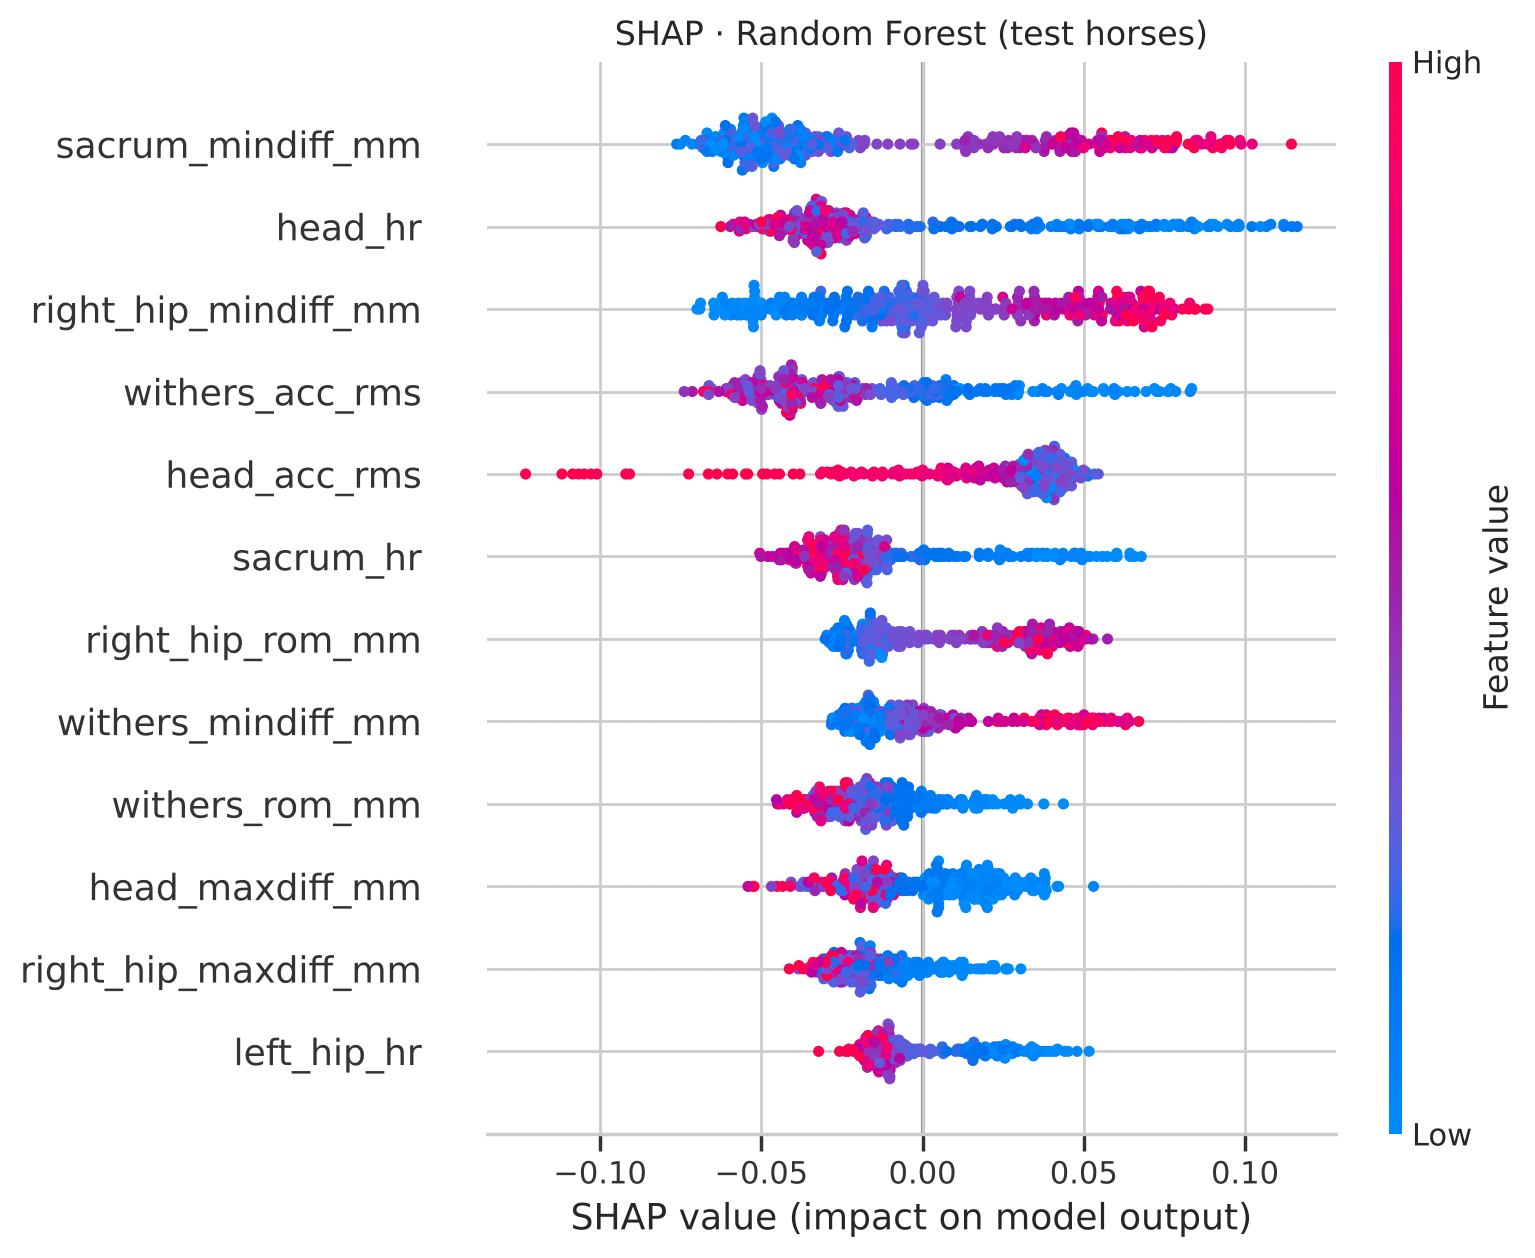
\includegraphics[width=0.85\columnwidth]{ml_shap_summary.png}
\caption{Most influential variables in the model according to SHAP.}
\label{fig:shap}
\end{figure}

\subsection{Scientific impact}

The linear models explained about 40\,\% of the variation in impact, the regularized polynomial regression around 50\,\% and the Random Forest somewhat more, due to its ability to capture interactions (Fig. 15). Ridge, Lasso and Elastic Net performed the same as linear regression, because with three thousand papers and few variables there was no overfitting to correct. Their main use was selecting variables. Lasso showed that the pose estimation, vision and cattle detection profiles, together with collaboration between countries, are associated with more citations per year, and that the classic clinical profiles are associated with fewer (Fig. 16). This reinforces the decision to orient the project towards computer vision.

\begin{figure}[!htb]
\centering
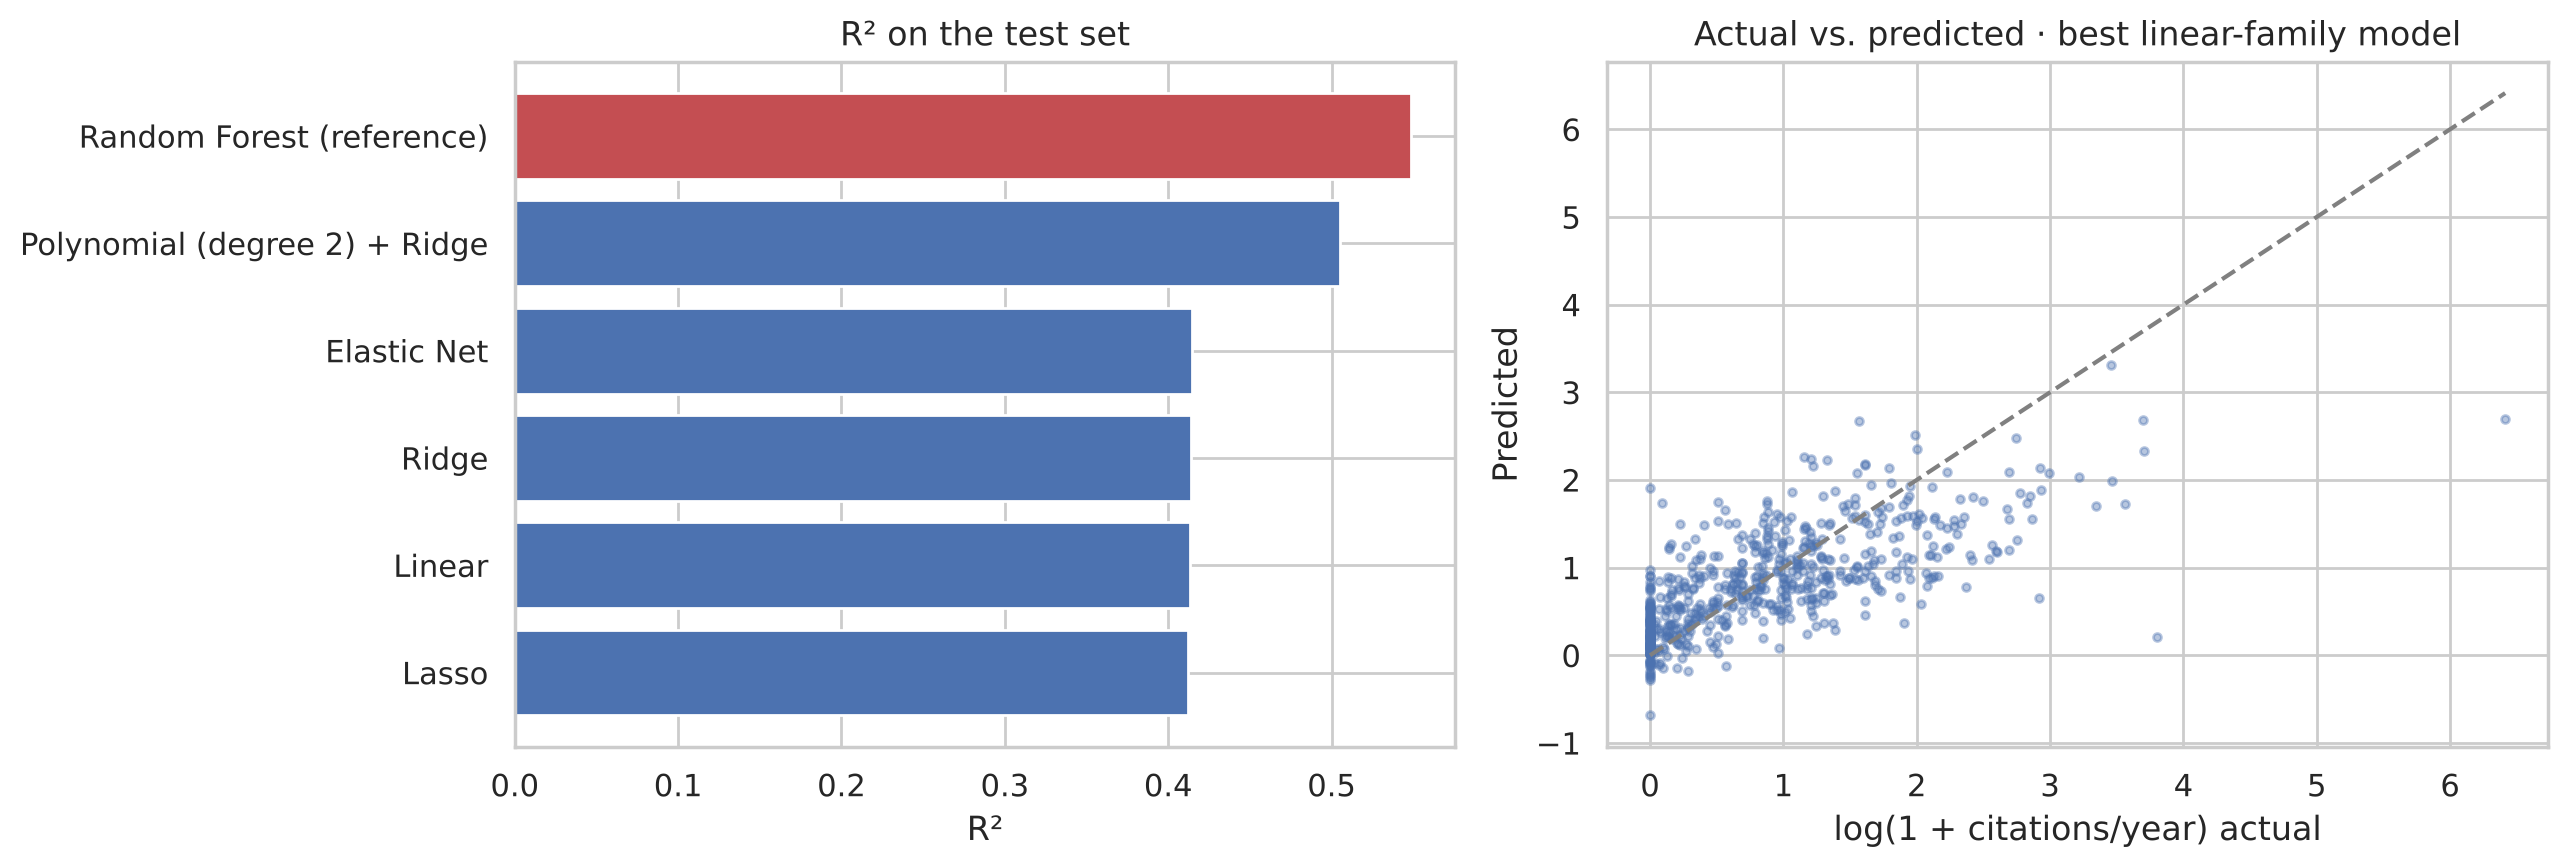
\includegraphics[width=\columnwidth]{reg_comparacion.png}
\caption{Comparison of regression models and actual versus predicted values.}
\label{fig:reg}
\end{figure}

\begin{figure}[!htb]
\centering
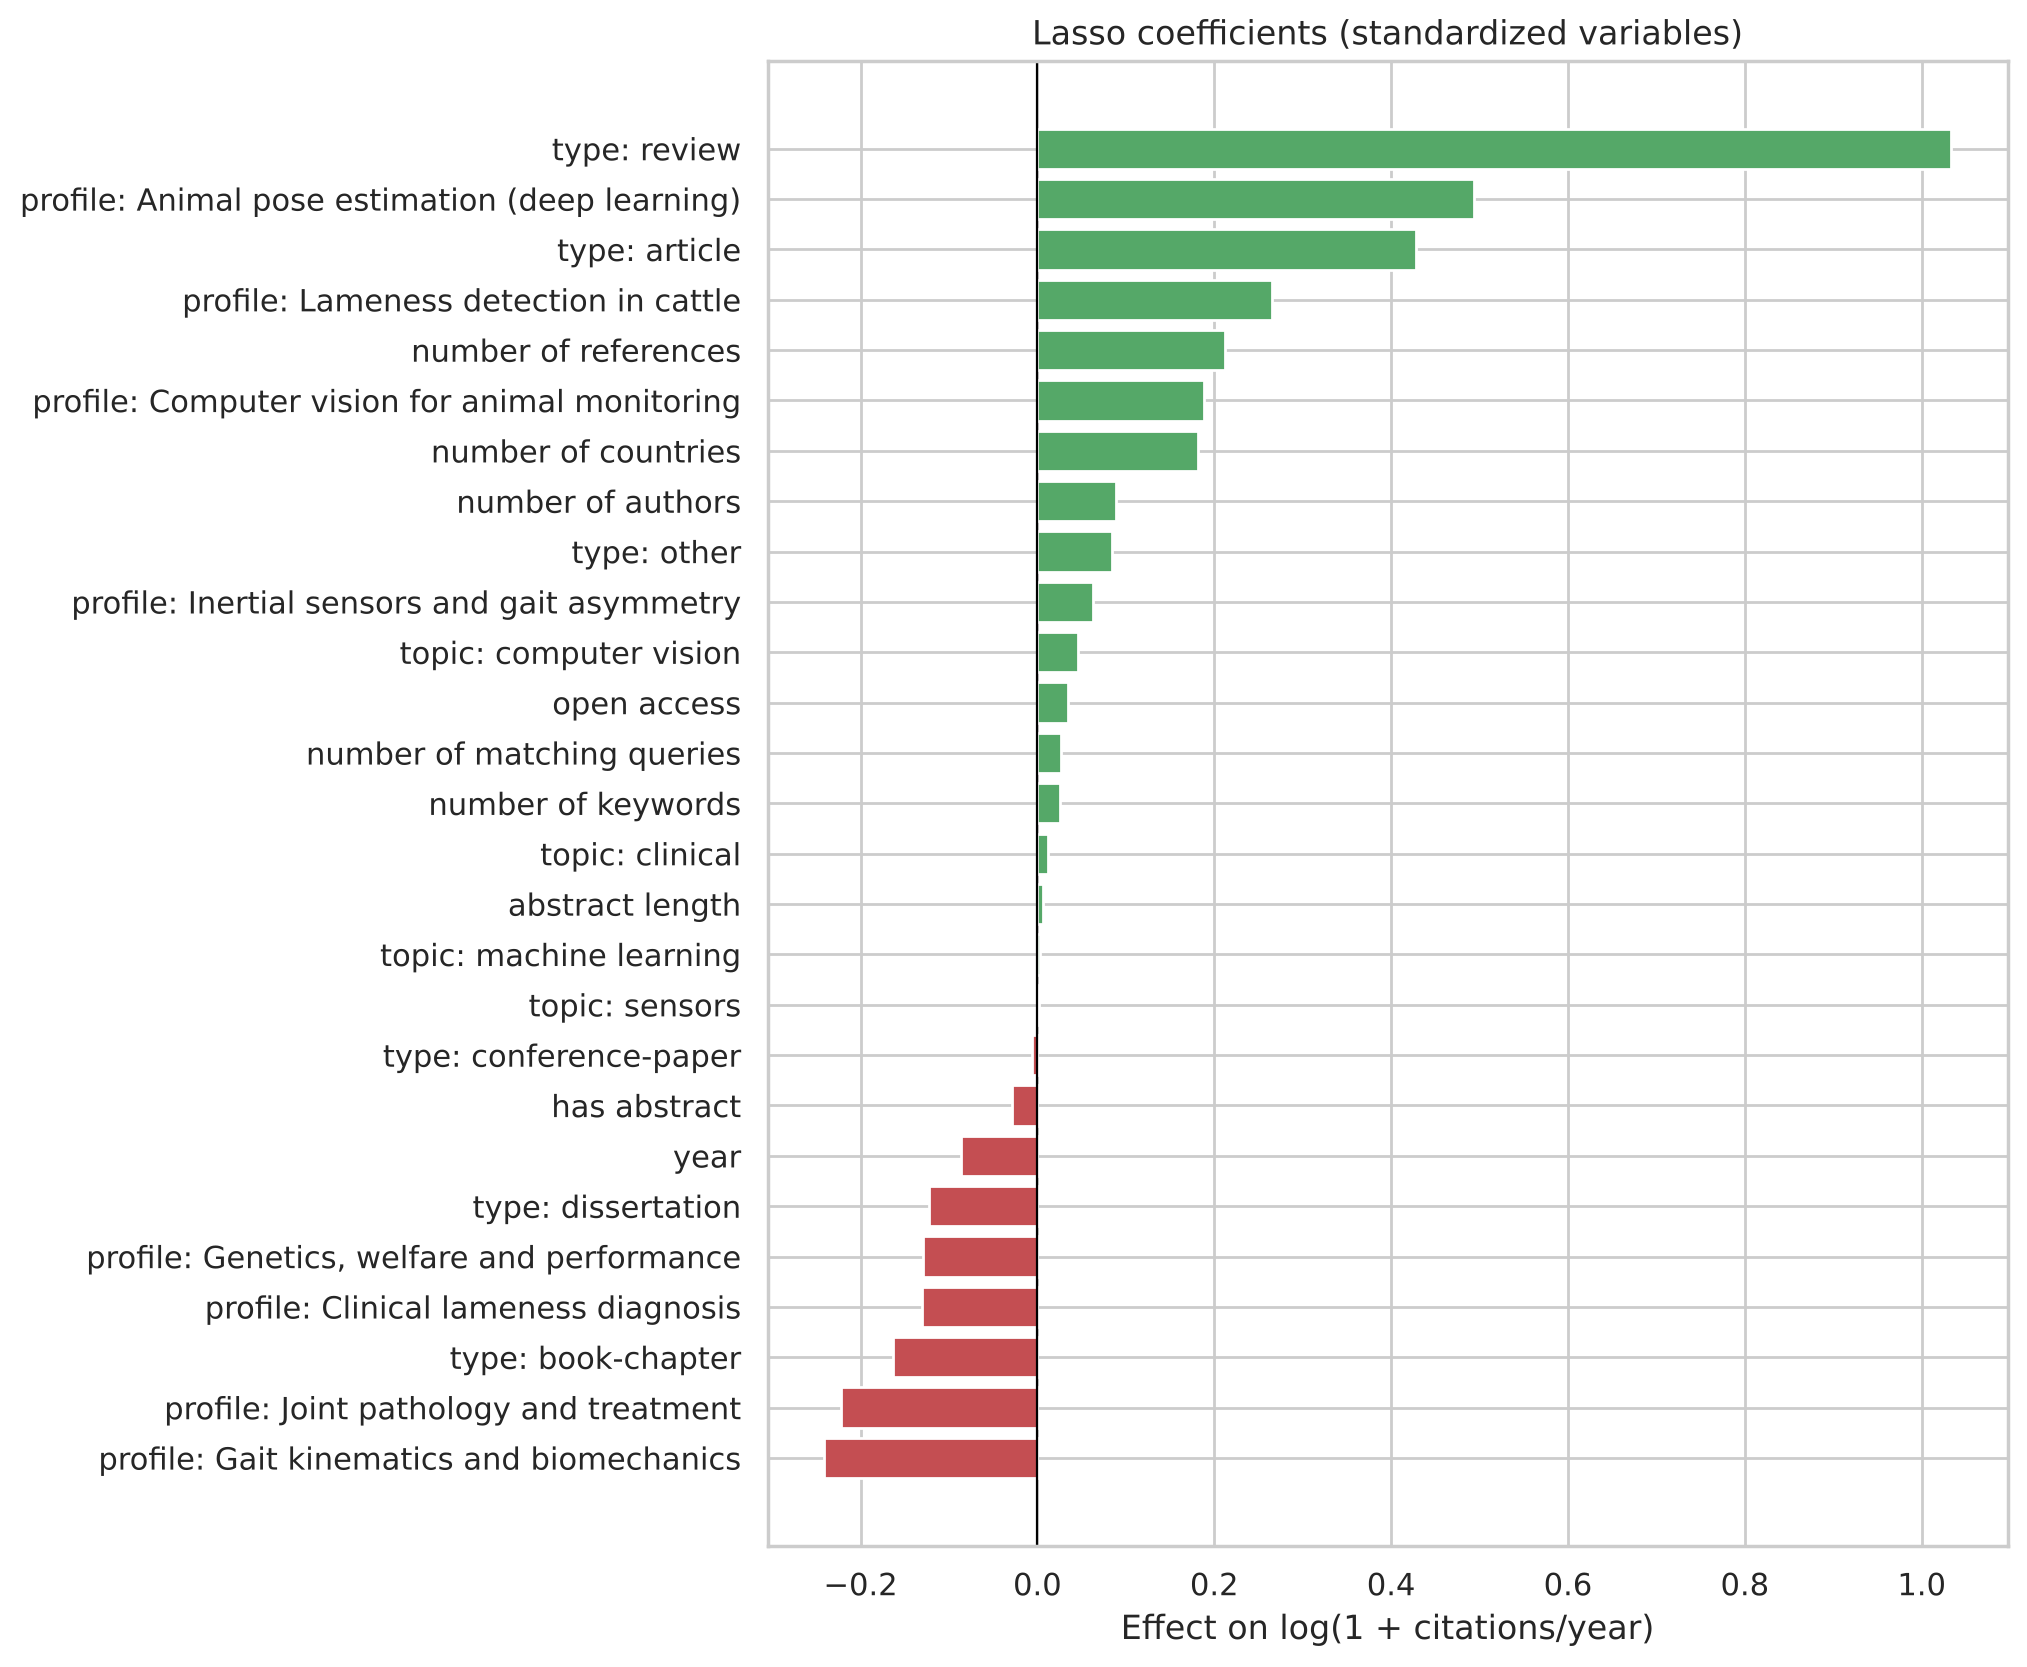
\includegraphics[width=0.9\columnwidth]{reg_lasso_coeficientes.png}
\caption{Lasso coefficients: characteristics associated with higher or lower impact of a paper.}
\label{fig:lasso}
\end{figure}

\section{Cost Analysis}

The estimate was made with list prices for the us-east-1 region for two scenarios (Table II). The academic scenario corresponds to the current use of the project and the pilot projects fifty clinics with twenty thousand trot trials per month. The academic cost is practically zero thanks to a serverless design. In the pilot the main weight is storage, and the architecture scales without changes. The actual cost, checked in the AWS billing console, has been zero dollars since deployment, because usage in these days was covered by the account's free tier, which is consistent with the estimate and confirms that the base of the system can operate at no cost in an academic context.

\begin{table}[!htb]
\centering
\caption{Estimated monthly cost in USD}
\label{tab:costos}
\begin{tabular}{lrr}
\toprule
Service & Academic & Pilot \\
\midrule
S3 and recovery replica & 0.17 & 9.80 \\
Lambda and API Gateway & 0.03 & 0.70 \\
DynamoDB and Athena & 0.03 & 1.46 \\
Parameter Store, ECR and CloudWatch & 0.15 & 1.55 \\
\midrule
\textbf{Total without free tier} & \textbf{0.38} & \textbf{13.51} \\
Total with free tier & 0.13 & 10.95 \\
\bottomrule
\end{tabular}
\end{table}

\section{Discussion}

The results answer the research question positively, although with nuances. Measures of head and pelvis asymmetry, which can be obtained with accessible technology, are enough to estimate the probability of lameness in horses the model does not know. In addition, the model relies on the same signs that the clinical literature associates with forelimb and hindlimb lameness~\cite{keegan2013}, which shows that it consistently learned a pattern present in nature.

On the other hand, the moderate performance of the resulting model is due to the following: the induced lameness was mild, precisely the case in which veterinarians themselves agree little~\cite{keegan2010,hammarberg2016}, and some horses already proved to be asymmetric while sound, which tends to confuse a general threshold.

The mining of the state of the art and the dataset catalogue also have a practical implication: moving to video requires obtaining the same trajectories from the image, replicating processes seen in the studies. At the same time, the lack of data with lameness labels and of studies in the region shows that a local contribution, with Criollo horses, would have scientific value. As for the cloud, the almost zero cost indicates that infrastructure is not a barrier to taking the system to a pilot.

\subsection{Limitations and future work}

The main limitations are the small number of horses, the use of induced rather than natural lameness, and a single breed. Future work includes comparing each horse with its own baseline, identifying the side of the asymmetry, estimating a lameness grade and, in the vision phase, computing these measures from video with a pose estimation model. In the longer term, it is proposed to collect our own data from Colombian Criollo horses assessed by veterinarians, whose gaits, such as paso fino and trocha, differ from the trot studied in the literature.

\section{Conclusions}

Data mining was crucial in this phase of the project, since it made it possible to map a field that is moving quickly towards computer vision and that leaves a clear gap: there are no open equine video data with lameness, and there is almost no Latin American research. In addition, the sensor data showed an asymmetry in the movement of the head and pelvis that reveals lameness in an interpretable way, and the model built on those measures works with horses it never saw. The complete system, from ingestion to prediction, was deployed in the cloud as code, at almost no cost. If in the next phase computer vision estimates those same trajectories from a video, the model and infrastructure of this work are ready to receive them.

\section*{Declaration of AI Use}

Claude (Anthropic) was used as a support tool for research tasks, document organization, writing review and code debugging. The author reviewed all the material and is responsible for its content.

\section*{Ethics and Data}

Only public data with open licences were used and no personal data were processed. The experimental protocol of the sensor dataset is the responsibility of its authors. The system is a support tool and does not replace the veterinary examination.

\begin{thebibliography}{99}
\bibitem{nehs2013} ``Equine health survey highlights the prevalence of lameness,'' \emph{Veterinary Record}, vol.~173, no.~6, p.~132, 2013, doi: 10.1136/vr.f4967.
\bibitem{usda1998} USDA APHIS, ``National economic cost of equine lameness, colic, and equine protozoal myeloencephalitis (EPM) in the United States,'' Info sheet, NAHMS Equine'98, Fort Collins, CO, USA.
\bibitem{keegan2010} K.~G. Keegan \emph{et al.}, ``Repeatability of subjective evaluation of lameness in horses,'' \emph{Equine Vet. J.}, vol.~42, no.~2, pp.~92--97, 2010, doi: 10.2746/042516409X479568.
\bibitem{hammarberg2016} M.~Hammarberg, A.~Egenvall, T.~Pfau, and M.~Rhodin, ``Rater agreement of visual lameness assessment in horses during lungeing,'' \emph{Equine Vet. J.}, vol.~48, no.~1, pp.~78--82, 2016, doi: 10.1111/evj.12385.
\bibitem{agronegocios2025censo} Agronegocios, ``¿Cuántos caballos hay en Colombia y de esta cifra cuántos están registrados?,'' 2025. [Online]. Available: \url{https://www.agronegocios.co/finca/cuantos-caballos-hay-en-colombia-y-de-esta-cifra-cuantos-estan-registrados-4206155}
\bibitem{un2015} United Nations, ``Transforming our world: the 2030 Agenda for Sustainable Development,'' Res. A/RES/70/1, 2015.
\bibitem{keegan2013} K.~G. Keegan \emph{et al.}, ``Comparison of a body-mounted inertial sensor system-based method with subjective evaluation for detection of lameness in horses,'' \emph{Am. J. Vet. Res.}, vol.~74, no.~1, pp.~17--24, 2013.
\bibitem{mathis2018} A.~Mathis \emph{et al.}, ``DeepLabCut: markerless pose estimation of user-defined body parts with deep learning,'' \emph{Nature Neuroscience}, vol.~21, pp.~1281--1289, 2018.
\bibitem{mathis2021} A.~Mathis \emph{et al.}, ``Pretraining boosts out-of-domain robustness for pose estimation,'' in \emph{Proc. IEEE/CVF WACV}, 2021, pp.~1859--1868.
\bibitem{li2024pferd} C.~Li \emph{et al.}, ``The Poses for Equine Research Dataset (PFERD),'' \emph{Scientific Data}, vol.~11, art.~497, 2024.
\bibitem{yu2021ap10k} H.~Yu \emph{et al.}, ``AP-10K: A benchmark for animal pose estimation in the wild,'' in \emph{NeurIPS Datasets and Benchmarks Track}, 2021.
\bibitem{yang2022apt36k} Y.~Yang \emph{et al.}, ``APT-36K: A large-scale benchmark for animal pose estimation and tracking,'' in \emph{NeurIPS Datasets and Benchmarks Track}, 2022.
\bibitem{ng2022animalkingdom} X.~L. Ng \emph{et al.}, ``Animal Kingdom: A large and diverse dataset for animal behavior understanding,'' in \emph{Proc. IEEE/CVF CVPR}, 2022, pp.~19023--19034.
\bibitem{ismail2024cow} S.~Ismail \emph{et al.}, ``CowScreeningDB: A public benchmark database for lameness detection in dairy cows,'' \emph{Comput. Electron. Agric.}, vol.~216, art.~108500, 2024.
\bibitem{wirth2000} R.~Wirth and J.~Hipp, ``CRISP-DM: Towards a standard process model for data mining,'' in \emph{Proc. 4th Int. Conf. Practical Applications of Knowledge Discovery and Data Mining}, 2000, pp.~29--39.
\bibitem{agrawal1994} R.~Agrawal and R.~Srikant, ``Fast algorithms for mining association rules,'' in \emph{Proc. 20th Int. Conf. Very Large Data Bases}, 1994, pp.~487--499.
\bibitem{han2000} J.~Han, J.~Pei, and Y.~Yin, ``Mining frequent patterns without candidate generation,'' in \emph{Proc. ACM SIGMOD}, 2000, pp.~1--12.
\bibitem{salton1988} G. Salton and C. Buckley, ``Term-weighting approaches in automatic text retrieval,'' \emph{Information Processing \& Management}, vol. 24, no. 5, pp. 513--523, 1988.
\bibitem{lloyd1982} S. Lloyd, ``Least squares quantization in PCM,'' \emph{IEEE Trans. Inf. Theory}, vol. 28, no. 2, pp. 129--137, 1982.
\bibitem{gower1971} J. C. Gower, ``A general coefficient of similarity and some of its properties,'' \emph{Biometrics}, vol. 27, no. 4, pp. 857--871, 1971.
\bibitem{liu2008} F. T. Liu, K. M. Ting and Z.-H. Zhou, ``Isolation forest,'' in \emph{Proc. IEEE Int. Conf. Data Mining (ICDM)}, 2008, pp. 413--422.
\bibitem{breiman2001} L.~Breiman, ``Random forests,'' \emph{Machine Learning}, vol.~45, no.~1, pp.~5--32, 2001.
\bibitem{friedman2001} J. H. Friedman, ``Greedy function approximation: A gradient boosting machine,'' \emph{Annals of Statistics}, vol. 29, no. 5, pp. 1189--1232, 2001.
\bibitem{lundberg2017} S.~M. Lundberg and S.-I. Lee, ``A unified approach to interpreting model predictions,'' in \emph{Advances in Neural Information Processing Systems 30}, 2017, pp.~4765--4774.
\bibitem{zou2005} H.~Zou and T.~Hastie, ``Regularization and variable selection via the elastic net,'' \emph{J. Royal Statistical Society: Series B}, vol.~67, no.~2, pp.~301--320, 2005.
\bibitem{tibshirani1996} R.~Tibshirani, ``Regression shrinkage and selection via the lasso,'' \emph{J. Royal Statistical Society: Series B}, vol.~58, no.~1, pp.~267--288, 1996.
\bibitem{mell2011} P. Mell and T. Grance, ``The NIST definition of cloud computing,'' NIST Special Publication 800-145, 2011.
\bibitem{terraform} HashiCorp, ``Terraform documentation,'' 2026. [Online]. Available: \url{https://developer.hashicorp.com/terraform/docs}
\bibitem{priem2022openalex} J.~Priem, H.~Piwowar, and R.~Orr, ``OpenAlex: A fully-open index of scholarly works, authors, venues, institutions, and concepts,'' arXiv:2205.01833, 2022.
\bibitem{smit2023dataset} I.~Smit \emph{et al.}, ``Kinematic data of the Icelandic horse with induced lameness at walk, trot and tölt,'' DataverseNL, 2025, doi: 10.34894/PEWAK6.
\end{thebibliography}

\end{document}
